\documentclass[a4paper,12pt, oneside]{book}

%\usepackage{fullpage}
\usepackage[T1]{fontenc}
\usepackage[italian]{babel}
\usepackage[utf8]{inputenc}
\usepackage{amssymb}
\usepackage{amsthm}
\usepackage{mathtools}
\usepackage{graphics}
\usepackage{amsfonts}
\usepackage{listings}
\usepackage{amsmath}
\usepackage{amstext}
\usepackage{engrec}
\usepackage{rotating}
\usepackage[safe,extra]{tipa}
\usepackage{showkeys}
\usepackage{multirow}
\usepackage{hyperref}
\usepackage{microtype}
\usepackage{enumerate}
\usepackage{braket}
\usepackage{marginnote}
\usepackage{pgfplots}
\usepackage{cancel}
\usepackage{polynom}
\usepackage{booktabs}
\usepackage{enumitem}
\usepackage{framed}
\usepackage{pdfpages}
\usepackage{pgfplots}
\usepackage[usenames,dvipsnames]{pstricks}
\usepackage{epsfig}
\usepackage{pst-grad} % For gradients
\usepackage{pst-plot} % For axes
\usepackage[space]{grffile} % For spaces in paths
\usepackage{etoolbox} % For spaces in paths
\makeatletter % For spaces in paths
\patchcmd\Gread@eps{\@inputcheck#1 }{\@inputcheck"#1"\relax}{}{}
\makeatother
\usepackage[cache=false]{minted}
\usepackage{fancyhdr}
\newcommand{\numberset}{\mathbb}
\newcommand{\N}{\numberset{N}}
\newcommand{\Z}{\numberset{Z}}
\newcommand{\Q}{\numberset{Q}}
\newcommand{\R}{\numberset{R}}

\pagestyle{fancy}
\fancyhead[LE,RO]{\slshape \rightmark}
\fancyhead[LO,RE]{\slshape \leftmark}
\fancyfoot[C]{\thepage}



\title{Probabilità e Statistica per l'Informatica}
\author{UniShare\\\\Davide Cozzi\\\href{https://t.me/dlcgold}{@dlcgold}\\\\Gabriele De Rosa\\\href{https://t.me/derogab}{@derogab} \\\\Federica Di Lauro\\\href{https://t.me/f_dila}{@f\textunderscore dila}}
\date{}

\pgfplotsset{compat=1.13}
\begin{document}
\maketitle
\tableofcontents

\definecolor{shadecolor}{gray}{0.80}

\newtheorem{teo}{Teorema}
\newtheorem{definizione}{Definizione}
\newtheorem{esempio}{Esempio}
\newtheorem{corollario}{Corollario}
\newtheorem{lemma}{Lemma}
\newtheorem{osservazione}{Osservazione}
\newtheorem{nota}{Nota}
\newtheorem{esercizio}{Esercizio}
\newcommand{\mean}[1]{\overline #1}
\renewcommand{\chaptermark}[1]{%
\markboth{\chaptername
\ \thechapter.\ #1}{}}
\renewcommand{\sectionmark}[1]{\markright{\thesection.\ #1}}
\chapter{Introduzione}
\textbf{Questi appunti sono presi a lezione. Per quanto sia stata fatta una revisione è altamente probabile (praticamente certo) che possano contenere errori, sia di stampa che di vero e proprio contenuto. Per eventuali proposte di correzione effettuare una pull request. Link: } \url{https://github.com/dlcgold/Appunti}.\\
\textbf{Grazie mille e buono studio!}

La statistica è una discliplina, basata sulla matematica, con finalità lo studio quantitativo e qualitativo
di un particolare fenomeno collettivo, in condizioni di incertezza o non determinismo ed è usata in molti 
ambiti, come ad esempio l'intelligenza artificiale, data science, robotica, domotica e tutte le analisi 
per poter ottenere ricavare delle informazioni sui dati.

Si ha l'\emph{A-B testing}, per decidere tra due scelte la migliore e per la decisione si analizzano i dati
presi da campioni di popolazione, utilizzando il \emph{tasso di conversione}, ossia la percentuale di visitatori unici
che hanno effettuato la azione su cui si sta effettuando il test.

In questo corso verranno affrontati e studiati i seguenti argomenti:
\begin{enumerate}
    \item statistica descrittiva
    \item calcolo delle probabilità
    \item distribuzioni notevoli
    \item teoremi di convergenza
    \item stima dei parametri
    \item test di ipotesi parametrici
    \item test di ipotesi non parametrici
    \item regressione lineare
\end{enumerate}

\chapter{Statistica Descrittiva}
La statistica descrittiva è una raccolta di metodi e strumenti matematici usati per organizzare una o più serie di dati
al fine di trovarne delle simmetrie, periodicità o delle eventuali leggi.

Solitamente i dati disponibili non rappresentano tutta la popolazione ma un numero limitato 
di osservazioni effettuato su un \emph{campione}, sottoinsieme selezionato della popolazione su cui si effettua
l'analisi statistica, la cui efficacia dipende da quale sottoinsieme è stato scelto, infatti non esiste 
un solo campione ma vi sono diversi modi per sceglierli, più o meno efficaci, per l'analisi statistica.

Quando si effettua un analisi statistica si vuole affermare qualcosa riguardo i \emph{caratteri} della popolazione,
ossia gli elementi su cui si effettua l'analisi statistica, che possono essere:
\begin{itemize}
    \item \emph{caratteri qualitativi}, indicanti qualità (colori, stili, materiali etc...) e anche dati non numerici
             in cui solitamente non è definita una \textit{relazione d'ordine}
    \item \emph{caratteri quantitativi}, maggiormente studiati dal corso, dati numerici 
          in cui vengono definite \emph{relazioni d'ordine}, che possono essere a loro volta divisi in
          \emph{discreti}, indicanti valori in $\Z$, e \emph{continui}, con valori nel campo $\R$.
\end{itemize}
Supponiamo di considerare $n$ elementi della popolazione e di rilevare, per ognuno di essi,
il dato relativo al carattere quantitativo da esaminare, ossia definiamo l'insieme di dati
$E=\{x_1, x_2, \dots, x_n\}$ con la numerosità, il numero di elementi considerati, pari a $n$.

In caso il carattere è discreto è comodo raggruppare i dati considerando l'insieme di tutti i valori assumibili,
detta \emph{modalità del carattere} ed associare ad ognuno di esso il numero di volte che esso compare in $E$.\newline
Si ha quindi il numero di totalità $N$ del carattere e si definisce l'insieme di modalita $S=\{s_1,...,s_N\}$
su cui si definiscono i seguenti valori statistici:
\begin{description}
    \item [frequenza assoluta ] numero di volte $f_j$ che si ha un elemento di un campione
    \item [frequenza cumulata assoluta] somma delle frequenze assolute di tutte le modalità, 
           indicato con $F_j$, calcolato con la seguente formula:
            \[ F_j = \sum_{k:s_k \leq s_j} f_k \]
    \item [frequenza relativa] rapporto tra la frequenza assoluta e il numero di elementi,
           indicata con $p_j$, calcolata come 
            \[ p_j = \frac{f_j}{n} \]
    \item [frequenza cumulativa relativa $P_j$] somma delle frequenze relativa di tutte le modalità,
           indicato con $P_j$, calcolata come 
            \[ P_j = \sum_{k:s_k \leq s_j} p_k \]
\end{description}
Si definisce \emph{distribuzione di frequenza} una funzione $F:S \to \N$ che associa ad ogni modalità 
la corrispondente frequenza, per cui esiste la distribuzione di frequenza assoluta, relativa, 
frequenza cumulativa assoluta e relativa.

%inserire esempio pagina 9
Quando il carattere da studiare è continuo o discreto con un gran numero di valori, è conveniente 
ricondursi a raggruppamenti come quelli appena trattati, per cui si suddivide l'insieme delle modalità $S$,
in alcune classi, sottoinsiemi di $S$, che formano una partizione.\newline
La scelta delle classi con cui si suddivide l'insieme $S$ è del tutto arbitraria anche se è necessario
che esse formino una partizione di $S$.\newline
Le partizioni devono essere significative e sufficientemente numerose ed inoltre ad ogni classe si associano le grandezze:
confini superiori ed inferiori, l'ampiezza e il valore centrale della classe.

Nel caso in cui il carattere esaminato sia continuo occorre specificare come le classi sono chiuse, a destra o a sinistra,
ossia specificare se gli elementi dell'indagine il cui dato coincide con il confine della classe sono da raggruppare
all'interno della classe stessa oppure no.
%esempio a pagina 13
\section{Indici di tendenza Generale}
Fino ad ora abbiamo visto come rappresentare i dati, ora iniziamo ad analizzare gli indici
che ci forniscono un valore che rappresenta un certo aspetto della serie di dati, 
incominciando dagli \emph{indici di tendenza generale}:
\begin{description}
    \item [media] è la media aritmetica tra tutti i valori dei dati osservati 
        \[ \overline{x} = \frac{1}{n} \sum _{i = 1} ^ n x_i = \frac{x_1 + \cdots + x_n}{n} \]
            Considerando le distribuzioni di frequenza definite, posssiamo fornire definizioni equivalenti di media:
                \[ \overline{x} = \frac{1}{n} \sum _{j = 1} ^ n s_j f_j = \sum s_j p_j \]
                La dimostrazione dell'uguaglianza di queste definizioni alternative è banale e si riconduce 
                alla definizione di frequenza relativa ed assoluta.

    \item [mediana] è l'elemento in mezzo ai valori dei dati, ordinati in maniera crescente
            in cui se il numero degli elementi $n$ è dispari è l'elemento $\frac{n + 1}{2}$
            altrimenti è la media degli elementi di posto $\frac{n}{2}$ e $\frac{n}{2} + 1$.

    \item [moda] valore o classe, indicato con $\widetilde{x}$, corrispondente alla massima frequenza assoluta
                 e viene usata solitamente in caso sia impossibile definire la media e la mediana.\newline
            La moda non è unica infatti parliamo di \emph{distribuzione uni-modale}, nel caso di un'unica moda,
            altrimenti di \emph{distribuzione multi-modale}.
\end{description}
%aggiungo esempio
Gli indici di tendenza centrale non sono utili per fornire informazioni circa l'omogeneità dei dati, in quanto forniscono 
informazioni sui valori centrali e medi del campione statistico, per cui per risolvere sto problema
introduciamo i seguenti indici:
\begin{description}
        \item [varianza] è la media dello scarto quadratico di ogni elemento dalla sua media 
                \[ s^2 = \frac{1}{n} \sum _{i = 1} ^ n (x_i - \overline{x})^2 \]
                La varianza ovviamente è tanto più grande quanto i singoli elementi si discostano dalla media, 
                ossia significa che i dati in tal caso sono molto disomogenei.\newline
                Come abbiamo già visto per la media sono presenti le seguenti definizioni alternative di varianza:
                \[ s^2 = \frac{1}{n} \sum _{j = 1} ^ N f_j (s_j - \overline{x}) ^ 2 \]
                \[ s^2 = \sum _{j = 1} ^ N p_j (s_j - \overline{x}) ^ 2 \]
                \[ s^2 = \sum _{j = 1} ^ n x_j - \overline{x} ^ 2 \]
                Le prime due definizioni alternative derivano dalla definizione di frequenza assoluta e frequenza 
                mentre l'ultima proviene da passaggi algebrici, dimostrati di seguito formalmente:
                \begin{proof}
                        \[ \begin{split}
                            s^2 & = \frac{1}{n} \sum _{i = 1} ^ n (x_i - \mean{x}) ^ 2 \\
                                & = \frac{1}{n} \sum (x_i ^ 2 - 2x_i\mean{x} + \mean{x} ^ 2) \\
                                & = \frac{1}{n} (\sum x_i^2 - 2\mean{x} \sum x_i + \sum \mean{x} ^ 2) \\
                                & = \frac{1}{n} (\sum x_i^2 - 2n\mean{x}^2 + n\mean{x}^2) \\
                                & = \frac{1}{n} \sum x_i^2 - \mean{x} ^ 2 \\
                            \end{split} \]
                Si dimostra $\sum x_i = n \mean{x}$ in quanto $\mean{x} = \frac{1}{n} \sum x_i$ e il resto 
                sono soltanto passaggi algebrici elementari
                \end{proof}

    \item [scarto quadratico medio] misura quanto sono distanti gli elementi di un campione ed è calcolata come:
            \[ s = \sqrt{s^2} = \sqrt{\frac{1}{n} \sum _{i = 1} ^ n (x_i - \overline{x}) ^ 2} \]
\end{description}
Nel calcolo della varianza si utilizza il quadrato per la differenza tra l'elemento e la sua media in quanto 
si ha $\sum (x_i - \overline{x}) = 0$, dato che la media è il valore la cui distanza è minima tra tutti gli 
elementi del campione.\newline
Per evitare questo problema si eleva la differenza tra un elemento e la sua media al quadrato.

La varianza è definito come il momento secondo rispetto alla media, come analizzeremo nel capitolo 3,
espresso tramite la formula:
\[ M_{k,y}=\frac{1}{n}\sum (x_i-y)^2 \]

Fino ad ora noi abbiamo considerato il caso unidimensionale ma molte analisi richiedono di analizzare
due o più caratteri del campione contemporaneamente, per riconoscere leggi ed analogie tra i diversi caratteri.\newline
Considereremo solo due caratteri contemporanei, sia perché un analisi con più caratteri si ha gli stessi
aspetti e sopratto per evitare di aggravare troppo la rappresentazione dei dati e assumiamo inoltre che 
entrambi i caratteri sono di tipo quantitativo e discreto, in quanto se fossero quantitativi continui
subirebbero prima un raggruppamento a classi.

L'insieme dei dati viene rappresentato come l'insieme delle coppie $E = \{(x_i, y_i) \,\,\,\forall i \leq n\}$
mentre l'insieme delle coppie di valori assumibili sono rappresentati con l'insieme
\[ S = \{(s_j, u_k), \, j = 1 \dots N \quad k = 1 \dots M\} \]
Come abbiamo fatto anche per il caso unidimensionale definiamo le seguenti quantità:
\begin{description}
    \item [frequenza assoluta ] è la quantita $f_{jk}$ corrispondente al numero di elementi con valore $(s_j, u_k)$
    \item [frequenza relativa] rapporto tra la frequenza e il numero di elementi, calcolato come 
          \[ p_{jk} = \frac{f_{jk}}{n} \]
    \item [frequenza cumulata assoluta] somma delle frequenze assoluta, calcolata come segue
           \[ F_{jk} = \sum _{r:s_r \leq s_j; l:u_l \leq u_k} f_{rl} \]
    \item [frequenza cumulata relativa] somma delle frequenza relative, calcolata come segue
           \[ P_{jk} = \sum _{r:s_r \leq s_j; u_l \leq u_k} p_{rl} \] frequenza 
\end{description}
Si definisce \emph{distribuzione di frequenza doppia} una qualsiasi funzione $f, F, p, P$ 
che associa ad ogni coppia $(s_j, u_k)$ la corrispondente frequenza ma non esistono solo queste funzioni,
infatti noi vediamo anche le \emph{distribuzioni marginali}, in cui si analizza la distribuzione dei singoli caratteri,
presi indipendemente dagli altri.

Le distribuzioni marginali hanno la definizione delle seguenti funzioni:
\begin{description}
    \item [frequenza assoluta marginale] quantità di elementi $f_xj$ data dagli elementi di $E$, 
                                         il cui primo carattere ha valore $s_j$
    \item [frequenza relativa marginale] rapporto tra la frequenza assoluta marginale e il numero di osservazioni $n$.
    \item [frequenza cumulata assoluta marginale] $F_{xj}$ somma delle frequenze assolute marginali 
                                                  di tutti gli $s_k$ con $s_k \leq s_j$
    \item [frequenza cumulata relativa marginale] $P_{xj}$ somma delle frequenze relative marginali
                                                  di tutti gli $s_k$ con $s_k \leq s_j$
\end{description}
Oltre a quelli definiti fino ad ora, esiste un indice che fornisce un grado di interdipendenza tra i due caratteri,
importante in quanto molti problemi concreti necessitano di analizzare gradi di correlazione tra due o più serie di dati,
iniziando prima di tutto da un esempio.

Considerando due serie $\{x_i\}$ e $\{y_i\}$, con $i = 1 \dots n$, e le coppie di scarti $x_i - \mean{x}$ 
e $y_i - \mean{y}$, di tutti i valori della serie rispetto alla media, si ha una relazione di dipendenza
tra i due caratteri se i due scarti corrispondono sistematicamente o quasi valori positivi o negativi.

Si definisce quindi la \textbf{covarianza} $c_{xy}$, dei dati o campionaria, come 
\[ c_{xy} = \frac{1}{n} \sum (x_i - \mean{x}) (y_i - \mean{y}) \]
La covarianza assume un valore positivo (negativo), che diviene grande in valore assoluto, nel caso in cui 
i termini prodotto abbiano segni concordi e in questo caso si parla di serie statistiche fortemente correlate
o per meglio dire di dati delle serie fortemente correlati.\newline
Nel caso opposto vale a dire nel caso in cui i dati delle serie siano incorrelati avremo che i prodotti
avranno segni diversi (saranno discordi in segno) e la covarianza, per come definita,
risulterà piccola in valore assoluto, prossima al valore 0.

Si ha anche la seguente formula per la covarianza:
\[ c_{xy} = \frac{1}{n} \sum x_iy_i - \overline{x}\overline{y} \]
\begin{proof}
        \[ \begin{split}
                c_{xy} & = \frac{1}{n} \sum _{i = 1} ^ n (x_i - \mean{x}) (y_i - \mean{y}) \\
                       & = \frac{1}{n} \sum _{i = 1} ^ n (x_iy_i - x_i\mean{y} - y_i \mean{x} + \mean{x}\mean{y}) \\
                       & = \frac{1}{n} (\sum x_iy_i - \mean{y} \sum x_i - \mean{x} \sum y_i + \sum \mean{x}\mean{y}) \\
                       & = \frac{1}{n} (\sum x_iy_i - n\mean{y}\mean{x} - n\mean{y}\mean{x} + n\mean{y}\mean{x}) \\
                       & = \frac{1}{n} (\sum x_iy_i - n\mean{x}\mean{y}) \\
                       & = \frac{1}{n} \sum x_iy_i - \mean{x}\mean{y} \\
            \end{split} \]
\end{proof}
Nel caso in cui i dati si riferiscano a caratteri quantitativi discreti, di cui è nota la
distribuzione di frequenza doppia, è possibile utilizzare le seguenti formule per il calcolo della covarianza:
\[ c{xy}=\sum_1^N\sum_1^M(s_j-\overline{x})(u_k-\overline{y})p_{jk} \]
\[c{xy}=\sum_1^N\sum_1^Ms_ju_kp_{jk}-\overline{x}\overline{y} \]

Date due serie di dati si ha le seguenti proprietà:
\begin{itemize}
    \item le due serie di dati \emph{statisticamente incorrelate} se la loro covarianza è nulla
    \item le due serie di dati sono \emph{statisticamente indipendenti} se vale:
        \[ \forall j=1, \dots, N\,\,k=1, \dots, M\,\,\, p_{jk} = p_jp_k \]
             con $p_{jk}$ frequenza relativa doppia mentre le altre sono le frequenze relative marginali.
\end{itemize}
Si ha che la proprietà di indipendenza è più forte dell'incorrelazione, infatti se le due serie di dati sono 
indipendenti, risultano anche incorrelate mentre il contrario non è detto, infatti risulta:
\[ \sum \sum (x_i - \overline{x})(y_i - \overline{y}) = \sum (x_i - \overline{x}) \sum(y_i - \overline{y}) = 0 \]
cosa che non è possibile leggerla al contrario.\newline
Nel caso bidimensionale, con variabili x e y, la covarianza si può rappresentare attraverso una matrice $2 \times 2$:
\[ C = \left | \begin{matrix}
                c_{xx} & c_{xy}\\
                c_{xy} & c_	{yy}
                \end{matrix}\right| = \left|\begin{matrix}
                                            var(x) & cov(x,y)\\
                                            cov(x,y) & var(y)
                                            \end{matrix}\right| \]
Per una misura indipendente dalla variabilità delle grandezze si usa la matrice di correlazione:
\[ Corr=\left|\begin{matrix}
              \frac{c_{xx}}{\sigma_x^2} & \frac{c_{xy}}{\sigma_x^2\sigma_y^2} \\
              \frac{c_{xy}}{\sigma_x^2\sigma_y^2}   & \frac{c_{yy}}{\sigma_y^2} 
              \end{matrix}\right|=\left|\begin{matrix}
                                            1 & corr(x,y)\\
                                            corr(x,y) & 1
                                        \end{matrix}\right| \]
che ovviamente può crescere in $m$ dimensioni.

\section{Regressione Lineare}
In molti casi ci si pone la questione se tra dei caratteri $x$ ed $y$ esista un legame/relazione di tipo funzionale
che ne descriva in modo soddisfacente corretto il legame realmente esistente.\newline
Si parla di un'\emph{analisi di regressione}, in caso in cui si considera ad uno dei due caratteri 
come variabile indipendente e si cerca una funzione che stabilisce la relazione tra i due caratteri.\newline
Se fisso $x$, come \emph{variabile indipendente}, cerco $y = f(x)$ in modo che essa descriva al meglio
il legame tra la variabile indipendente $x$ e il carattere $y$, che a questo punto viene 
interpretato come \emph{variabile dipendente}.

Si determina quindi la funzione $f$ che minimizza le distanze tra i valori osservati del carattere $y$
e quelli ottenibili se la relazione tra $x$ e $y$ fosse proprio quella descritta da $f$, 
quindi si cerca la funzione $f$ che minimizza la quantità:
\[ g(f) = \sum[f(x_i)-y_i]^2 \]
dove il quadrato si utilizza affinché le distanze vengano tutte considerate con segno positivo.\newline
Se $f$ è vincolata ad essere una funzione lineare allora si parla di \textbf{regressione lineare}, 
con la retta rappresentata da $y=mx+q$, tale per cui risulti minima la quantità:
\[ g(m,q) = \sum[mx_i+q-y_i]^2 \]
con $mx_i+q=f(x_i)$ che sono l'approssimazione alle $y_i$ mediante $f$.\newline
Si ha che:
\[ m = \frac{c_{xy}}{s^2_x} \]
\[ q = \overline{y} - \frac{c_{xy}}{s_x^2}\overline{x} \]
Questo metodo consente di determinare la retta che meglio descrive la relazione tra i due caratteri 
senza peraltro fornire alcuna indicazione circa il grado di approssimazione che è in grado di offrire.\newline
Per tale motivo è stata introdotta una nuova grandezza detta \textbf{coefficiente di correlazione lineare:}
\[ r_{xy}=\frac{c_{xy}}{s_xs_y} \]
L'importanza di tale coefficiente deriva dal fatto che esso assume valori sempre appartenenti all'intervallo $[-1, 1]$ 
ed inoltre il coefficente è nullo se le serie sono statisticamente incorrelate.\newline
il valore assoluto risulta tendente a 1 se le coppie sono tutte sulla retta $y=mx+q$,
quindi rappresenta il grado di allineamento delle coppie di dati.

Abbiamo accennato in precedenza al fatto che non si è sempre vincolati alla scelta di una retta tra le funzioni
che possono descrivere la relazione tra le due serie di dati ma quanto esposto in precedenza può essere applicato 
anche nel caso in cui si considerino relazioni funzionali di diversa natura, la cui scelta può essere suggerita
da una qualche impressione derivante da ispezioni visive dei dati o da altre forme di conoscenza circa il fenomeno analizzato,
avendo quindi il modello non lineare di regressione.

Molte relazioni funzionali non lineari possono essere ricondotte a tali (lineari) con opportune trasformazioni delle variabili,
infatti prendendo per esempio la relazione:
\[ y = a\cdot e^{bx} \]
che si può riscrivere come:
\[ \widetilde{y} = \beta\cdot \widetilde{x}+\alpha \]
con: 
\[ \widetilde{y}=\log(y) \]
\[ \widetilde{x}=x \]
\[ \alpha=\log(a) \]
\[ \beta = b \]
si ottiene quindi una sorta di curva e non più una retta.

La determinazione dei coefficienti a e b che meglio permettono di approssimare una serie di punti $\{x_i,y_i\}$ 
può essere effettuata riconducendosi ad una regressione lineare ovvero determinando i coefficienti $\alpha,\beta$ 
che meglio approssimano, linearmente, la serie dei punti $\{\widetilde{x}_i,\widetilde{y}_i\}$, con:
\[ \widetilde{y}_i = \log(y_i) \]
\[ \widetilde{x}_i = x_i \]
Una volta determina ti tali coefficienti il calcolo di $a$ e $b$ risulta immediato. 

Ecco alcune funzioni riconducibili a lineari:
\[ y = a \log(x) + b \]
\[ y=ax^b \]
\[ y=\frac{1}{a+b\cdot e^{-x}} \]

\chapter{Calcolo delle probabilità}
La probabilità è la disciplina di carattere matematico che permette di affrontare l'analisi 
delle situazioni che hanno un esito imprevedibile a priori e pertanto con conseguenze incerte 
ed è lo strumento di base della statistica, che invece trae conclusioni
su una popolazione, utilizzando i dati osservati su una collezione di individui appartenenti alla popolazione,
basandosi inoltre su considerazioni probabilistiche.

Si hanno 4 impostazioni per la probabilità:
\begin{enumerate}
    \item \emph{classica}, in cui la probabilità di un evento $A$ è data dal rapporto tra i casi favorevoli e il
          numero di casi possibili, supponendo tutti i casi ugualmente possibili.
    \item \emph{frequentista}, in cui la probabilità di un evento è il limito del rapporto tra gli esperimenti
          favorevoli all'evento e il totali di quelli effettuati, supponendo di averli ripetuti nella stessa
          condizione.
    \item \emph{soggettivista}, in cui la probabilità di un evento è la misura del grado di fiducia che un individuo
          attribuisce al verificare dell'evento $A$ e questa impostazione è basata su quanto uno scommettitore
          pagherebbe per il verificare dell'evento.
    \item \emph{assiomatica}
\end{enumerate}
Iniziamo a considerare l'impostazione assiomatica, supponendo di voler studiare una situazione con un insieme $\Omega$
,detto \emph{spazio campione}, di possibili esiti ben distinti tra loro, in cui tutti i suoi sottoinsiemi $A$
sono eventi, elementari in caso contengono solo un elemento altrimenti sono composti,
e ad ogni evento si ha una quantità numerica $P(A)$ detta \emph{probabilità}.

Un passo fondamentale nel superare le polemiche sull'interpretazione del concetto di probabilità
fu compiuto da Kolmogorov (1933) che abbandonò il tentativo di fondare la teoria della probabilità su una 
interpretazione sperimentale del concetto e costruire una teoria secondo una \emph{impostazione assiomatica},
trascendendo il significato effettivo di probabilità, rinviandone l'interpretazione al momento delle applicazioni.

Due eventi sono \emph{incompatibili} se non hanno elementi in comune, formando un intersezione vuota
e l'insieme delle parti di $\Omega$, $\wp(\Omega)$, definisce ovviamente l'insieme di tutti i sottoinsiemi.

Si dice \emph{misura di probabilità} ogni applicazione $P: \wp(\Omega) \to \R_0 ^ +$
che associa un valore reale ad ogni sottoinsieme di $\Omega$ e per cui valgono le seguenti proprietà:
\begin{itemize}
        \item esiste ed è un unico numero $P(A) \geq 0 \quad \forall A \subseteq \Omega$
        \item $P(\Omega) = 1$ 
        \item data la famiglia $\{A_i\in I\subseteq N\}$ di eventi incompatibili vale:
                \[ P\left(\bigcup_{i\in I}A_i\right) = \sum_{i\in I} P(A_i) \]
\end{itemize}
Ogni misura di probabilità è una funzione che assegna valori numerici a sottoinsiemi di $\Omega$
e non ai suoi elementi, come contrariamente si è portati a credere intuitivamente,
infatti avviene che la funzione di misura di probabilità associa un valore agli eventi elementari
come una conseguenza dell'assegnazione di valori ad eventi composti.\newline
La definizione di probabilità non fornisce indicazioni su quali valori numerici devono essere assegnati dato che dipende,
come sempre dal particolare problema da analizzare.

Dalla definizione assiomatica derivano facilmente le seguenti proprietà aggiuntive:
\begin{definizione}
Sia P una misura di probabilità definita sull'insieme delle parti $\wp(\Omega)$ di uno
spazio campione $\Omega$ allora:
    \begin{itemize}
        \item $\forall A, B \subseteq \Omega \mbox{ eventi anche incompatibili}$ risulta che
                $P(A \cup B) = P(A) + P(B) - P(A \cap B)$
                \begin{proof}
                 Si dimostra che:
                \[ P(A \cup B) = P(A \cap \overline{B}) + P(A \cap B) + P(\overline{A} \cap B)\]
                 Si ricava e si sa che sono soddisfatte le seguenti equazioni
                 \[P(A) = P(A \cap \overline{B}) + P(A \cap B) \]
                 \[P(B) = P(A \cap B) + P(\overline{A} \cap B) \]
                        quindi si ricava dall'equazione iniziale, sostituendo $P(A)$ e $P(B)$ la seguente equazione:
                    \[P(A \cup B) = P(A) + P(B) - P(A \cap B)\]
                \end{proof}
        \item $\forall A \subseteq \Omega \to P(\overline{A}) = 1 - P(A)$
              \begin{proof}
                    \[  \forall A\subseteq \Omega \to P(\overline{A})=1-P(A)\]
                        \[\downarrow\]
                    \[ 1 = P(A \cup \overline{A} )= P(A) + P(\overline{A}) - P(A \cap \overline{A}) = P(A) + P(\overline{A}) - 0\]
              \end{proof}
        \item $\forall A\subseteq \Omega$ risulta che $ P(A)\leq 1$
        \item $\forall A,B\subseteq \Omega, A\subseteq B$ risulta che $P(A)\leq P(B)$
    \end{itemize}
\end{definizione}
Si ha che il terzo assioma della probabilità generalizza la definizione di $P(A \cup B)$,
nel caso di tutti gli eventi incompatibili, mentre la terza e la quarta proprietà si dimostrano facilmente,
considerando gli elementi basilari di teoria degli insiemi e dei 3 assiomi della probabilità.

Si ha uno spazi campione con elementi equiprobabili se dato $\Omega = \{1, 2, \dots, N\}$ tale che:
\[P(\{1\}) = \dots = P(\{N\}) = p \]
Da questa formula si ricava facilmente le seguenti due equazioni, fondamentali per il calcolo della probabilità:
\[P(\{1\}) + \dots + P(\{N\}) = Np = p(\Omega) = 1\]
\[P(\{i\}) = p = \frac{1}{n}\]
Da quest'ultima equazione, considerando anche il terzo assioma della probabilità si ricava che la probabilità
di evento $E$ è data dal rapporto tra i numeri degli eventi elementari dell'elemento e la numerosità degli
elementi dello spazio campione.\newline
Si ha inoltre che la probabilità di un evento $E$ è data dalla seguente formula
\[ P(E) = \frac{\mbox{num. eventi elementari} E}{N} \]

In caso si facciano due esperimenti: se l'esperimento 1 può avere n possibili esiti equiprobabili,
e l'esperimento 2 può avere m possibili esiti equiprobabili, allora i due esperimenti hanno $n\times m$ possibili esiti.\newline
Se si espande a $r$ esperimenti si avranno $n_1\times n_2\times ...\times n_r$ possibili esiti, come 
tutti sappiamo dalla regola del prodotto del calcolo combinatorio.

\section{Accenni di Calcolo Combinatorio}
\begin{definizione}
    Si definisce permutazione di $n$ oggetti $a_1, a_2, \dots, a_n$ un ordinamento degli $n$ oggetti
    e il numero di permutazioni possibili in un insieme di $n$ oggetti è uguale a $n!$.
\end{definizione}
Dato un insieme di $n$ elementi, per calcolare il numero di modi di scegliere $k$ elementi dall'insieme
di $n$ elementi, senza possibilità di ripetizione, vi sono due modi:
\begin{itemize}
    \item \emph{disposizione semplice}, quando è importante l'ordine di scelta degli elementi e viene
        calcolato come segue
        \[ D(n, k) = n * (n - 1) * (n - 2) * \dots * (n - k + 1) \]
        Questa definizione è molto intuitiva, infatti il primo elemento può essere scelto tra $n$ elementi,
        il secondo tra $n-1$ elementi e così via fino ad arrivare a prelevare da $n - (k-1)$ elementi.
    \item \emph{combinazioni semplici}, quando l'ordine tra gli elementi scelti è irrilevante e si utilizza
          come simbolo $\binom{n}{k}$, che indica il numero di sottoinsiemi di $k$ elementi scelti
          dall'insieme con cardinalità $n$.\newline
          Il coefficente binomiale, come si dovrebbe conoscere da altri corsi, si calcola come
          \[ \binom{n}{k} = \frac{D(n, k)}{k!} = \frac{n!}{k! (n-k)!} \]
          Dalla definizione e dal significato di $\binom{n}{k}$ appare chiaro che 
          \[ \binom{n}{0} = 1 = \binom{n}{n} \quad \binom{n}{1} = n \]
          Valgono inoltre anche le seguenti proprietà:
          \[ \binom{n}{k} = \binom{n}{n-k} \]
          \[ \binom{n + 1}{k} = \binom{n}{k} + \binom{n}{k - 1}\]
          Quest'ultima formula ci permette di definire il triangolo di tartaglia, che tutti gli studenti
          scientifici ed informatici dovrebberò già conoscere, e di inoltre $\binom{n}{k}$ si chiama 
          \emph{coefficiente binomiale} perchè compaiono come coefficiente nella formula di Newton, per 
          calcolare lo sviluppo di un binomio $(x + y)^n$, come si può notare
          \[ (x + y)^n = \sum _{i = 0} ^ n \binom{n}{k} x^{n-k} y^k\]
\end{itemize}

\section{Probabilità condizionata}
In molti casi, quando si desideri studiare un fenomeno con comportamenti aleatori, oppure si vuole effettuare
un esperimento con esiti imprevidibili a priori, si utilizzano alcune informazioni complementari per restringere 
il campo dei possibili risultati e per poter trattare matematicamente queste situazioni viene introdotto
il concetto di \emph{probabilità condizionata}.

\begin{definizione}
Siano dati uno spazio campione $\Omega$ ed una misura di probabilità P definita su $\wp(\Omega)$ e
secondo l'impostazione assiomatica di probabilità, considerati due eventi, A e B con $P(B)>0$,
viene definita  probabilità dell'evento A condizionata dall'evento B la quantità:
\[P(A|B) = \frac{P(A\cap B)}{P(B)} \]
\end{definizione}
Questa definizione non è limitata solo alla probabilità assiomatica, infatti secondo l'approccio frequentista 
si definisce la probabilità dell'evento A, limitandosi a considerare solo i casi appartenenti a B come totale dei casi possibili.

Con la probabilità condizionata vi possono essere 3 diversi casi:
\begin{itemize}
    \item la probabilità dell'evento B sotto condizionamento diviene maggiore rispetto a quella 
          che avrebbe assunto senza condizionamento
    \item il valore di probabilità diminuisca a fronte del condizionamento
    \item può accadere che il condizionamento rispetto ad un evento non inficia in alcun modo la probabilità di 
        un altro evento ed in sto caso i due eventi sono \emph{stocasticamente indipendenti}.
\end{itemize}
Due eventi $A, B \in \wp(\Omega)$ sono stocasticamente indipendenti in caso in cui $P(A) = P(A | B) = P(B)$
da cui risultano i seguenti risultati:
\begin{itemize}
    \item $P(A \cap B) = P(A) P(B)$
    \item $P(A \cap B) = P(A | B) P(B)$
\end{itemize}
L'ultima formula presentata può essere generalizzata ad $n$ eventi, venendo chiamata 
\emph{formula del prodotto}, nel seguente modo:
\begin{definizione}
    Sia $n \in \N _+$ e data la famiglia $\{A_i i=1, \cdots, n\}$ di sottoinsiemi di $\Omega$, allora risulta
    \[P(A_1 \cap A_2 \cap \cdots \cap A_n) = P(A_1) P(A_2 | A_1) P(A_3 | A_1 \cap A_2) \cdots 
                                             P(A_n | A_1 \cap A_2 \cap \cdots \cap A_{n-1}) \]
\end{definizione}
Considerata una partizione dello spazio campione $\Omega$, si hanno le seguenti formule:
\begin{itemize}
    \item $P(B) = \sum_{i = 1} ^ n P(B | A_i) P(A_i)$ (formula delle probabilità totali)
    \item $P(A_i | B) = \frac{P(B | A_i) P(A_i)}{\sum_{i = j} ^ n P(B | A_j) P(A_j)}$ (formula di Bayes)
\end{itemize}

\section{Variabili Aleatorie}
In base a quanto visto fino ad ora per affrontare problemi di calcolo delle probabilità occorre di volta
in volta definire in maniera appropriata lo spazio campione e la misura di probabilità.\newline
Questo fatto comporta delle difficoltà se ci si pone come obiettivo la formulazione di una teoria
generale della probabilità, in quanto spazio campione e misura di probabilità sono diversi ogni volta ed
inoltre in quasi tutti i problemi concreti si ha a che fare con situazioni il cui esito, 
imprevedibile a priori, è di tipo numerico.

Queste considerazioni hanno portato i matematici ad introdurre delle opportune trasformazioni,
chiamate \emph{variabili aleatorie}, che consentono di ricondursi sempre ad $\R$ come spazio campione
ed a considerare quali suoi sottoinsiemi tutti gli intervalli del tipo $(a,b)$ o $[a,b]$ 
con $-\infty \leq a < b \leq +\infty$ in cui sono comprese tutte le possibili unioni ed intersezioni, 
finite o infinite, e i loro complementi.

Dato uno spazio campione $\Omega$ si definisce \emph{variabile aleatoria o casuale} un'applicazione $X:\Omega \to \R$
che associa un numero reale ad ogni elemento di $\Omega$.\newline
In base a questa definizione è possibile assegnare delle probabilità ad eventi del tipo $X \in B \subseteq \R$ in quanto
\[ P(X \in B) = P(\{\omega \in \Omega : X(\omega) \in B\}) \]
ma ciò appesantisce troppo la notazione per cui utiliziamo per comodità $P(X \in B)$ con però $X \in B$ un evento in $\Omega$,
invece di rappresentare la funzione della variabile aleatoria.

Dal punto di vista intuitivo la definizione di variabile aleatoria è poco chiara ma nel nostro caso assumiamo,
senza andare ad affrontare in maniera dettagliata, che essa rappresenta le quantità d'interesse determinate
dall'esecuzione dell'esperimento su cui si vuole conoscere la probabilità di avvenimento dell'evento.

Come notazione adotteremo quella solitamente utilizzata in campo statistico,
indicando con lettere maiuscole le variabili aleatorie e con lettere minuscole le rispettive possibili realizzazioni.\newline
Essendo imprevedibile a priori il valore assunto da una variabile aleatoria, tutto ciò che si può fare 
relativamente ad essa è esprimere delle valutazioni di tipo probabilistico sui valori che essa assumerà
e per tale ragione ad ogni variabile aleatoria X è associata una funzione, la \emph{funzione di ripartizione}
$F_X: \R \to [0, 1] \subset \R$ definita come:
\[ F_X(t) = P(X \leq t) \quad \forall t \in \R \]
che ci indica la probabilità che la variabile casuale $X$ assuma un valore minore o uguale a $t$.

Come si può notare nella \figurename~\ref{img:ripartizione}, la funzione di ripartizione è una funzione a gradini,
in cui ad ogni valore intero si ha la presenza di un punto di discontinuità, con un salto in avanti.

\begin{figure}
    \centering
    \caption{Funzione di ripartizione}
    \label{img:ripartizione}
    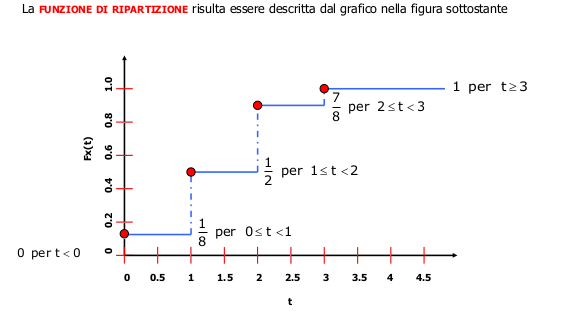
\includegraphics[scale=0.8]{img/rip.png}
\end{figure}
Avendo definito la funzione di ripartizione, adesso tutte le questioni riguardanti la variabile casuale $X$
possono trovare una soluzione attraverso di essa, infatti supponiamo di calcolare $P(\{a < X \leq b\})$
con l'evento ${X \leq b}$ esprimibile come l'unione dei due eventi indipendenti ${X \leq a}$ e ${a < X \leq b}$ 
da cui si ricava, usando il terzo assioma della probabilità la seguente formula:
\[ \begin{split}
        P(\{X \leq b\}) & = P(\{X \leq a\}) + P(\{a < X \leq b\}) \ \text{da cui si ricava} \\
        P(\{a < X \leq b\}) & = F(b) - F(a) \\
    \end{split} \]
Questa formula ci permette di determinare la probabilità che una variabile casuale possa assumere valori in intervalli reali
e ciò ha un notevole utilizzo in statistica e nella probabilità.

In genere la funzione di ripartizione non è nota, altrimenti tutti gli eventi della nostra vita sarebbero facilmente analizzabili
senza nessuna incertezza, ossia ad esempio si sarebbe in grado di prevedere come vincere al superenalotto e
tutti i giochi d'azzardo,  per cui l'obiettivo della statistica è di determinarla o determinare le grandezza ad essa associate
mentre la probabilità e le sue applicazioni assumono che essa sia  sempre nota.

Si dimostra che sono delle funzioni di ripartizione tutte e sole le funzioni del tipo $F: \R \to [0, 1]$
che godono simultaneamente delle seguenti proprietà:
\begin{itemize}
    \item $F$ è monotona crescente
    \item $\lim_{t \to +\infty} F(t) = 1$
    \item $\lim_{t \to -\infty} F(t) = 0$
    \item $\lim_{t \to t_0 ^ +} F(t) = F(t_0),\,\,\forall t_0 \in \R$
\end{itemize}
Le variabili aleatorie si distinguono in due categorie, in base a che valori può assumere 
l'insieme di valori $S$ di supporto:
\begin{itemize}
    \item \emph{variabili aleatorie discrete}: l'insieme $S$ è finito oppure costituito da un insieme
                                               infinito di valori discreti.
    \item \emph{variabili aleatorie continue}: l'insieme $S$ assume valori infiniti continui
\end{itemize}
Iniziamo ad analizzare prima le variabili discrete, più semplici da analizzare per poi considerare il caso
continuo, in cui si estendono i valori assumibili dalle variabili.

\subsection{Variabile Aleatoria Discreta}
Come già visto, una variabile aleatoria è detta \emph{variabile aleatoria discreta} nel caso in cui l'insieme dei valori $S$
che essa può assumere  è finita oppure da un infinito di valori discreti, in cui si associa anche, oltre alla
funzione di ripartizione, una funzione di probabilità assunta da valori specifici.\newline
Sia $S$ il supporto della variabile aleatoria $X$ e si definisce \emph{distribuzione discreta di probabilità} la funzione:
$p_X:\R \to [0,1]$ così definita:
\[
    p_X = \begin{cases}
            P(X = t)& \forall t \in S\\
            0& \mbox{ altrimenti}\\
          \end{cases}\]
Una funzione rappresenta una distribuzione di probabilità, in caso siano soddisfatte entrambe le seguenti proprietà:
\begin{itemize}
    \item \[ p_X(t) \geq 0 \quad \forall t \in R \]
    \item \[ \sum _{s \in S} p_X(s) = 1 \]
\end{itemize}
Tra le funzioni di ripartizione e le distribuzioni discrete esiste una corrispondenza biunivoca, in quanto
si hanno le seguenti equivalenze:
\begin{itemize}
    \item \[F_X(t) = \sum _{s \in S:s \subseteq t} p_X(s)\,\,\, \forall t \in \R\]
    \item \[p_X(s) = F_X(s) - \lim _{t \to s^{-}} F_X(t)\,\,\, \forall s \in S\]
\end{itemize}
Dalla prima di tali relazioni se ne deduce che le funzioni di ripartizione delle variabili
aleatorie discrete presentano dei \textit{salti} in corrispondenza dei valori \textit{s} mentre
sono costanti per gli altri valori, come si può anche notare nella figura ~\ref{img:ripartizione}

\subsection{Variabile Aleatoria Continua}
Come già affermato in precedenza, una variabile aleatoria è detta continua nel caso in cui la 
corrispondente funzione di ripartizione $F_X$ sia continua, ed in particolare viene detta 
\emph{assolutamente continua} se esiste una funzione $f_X:\R \to \R_+$ tale che
\[F_X(t) = \int _{-\infty}^t f_X(u)du \,\,\, \forall t \in \R\]
Una tale funzione, in caso in cui è definito l'integrale, viene detta \emph{densità di probabilità }di $X$.

È detto poi \emph{supporto} della variabile $X$ l'insieme $S = \{t \in \R : f_X(t) \neq 0\}$
e si osservi che se la densità di probabilità esiste allora la sua funzione di ripartizione è una sua
primitiva.

Per semplicità supporremo nel seguito che le variabili aleatorie assolutamente continue abbiano funzione
di ripartizione derivabile e che la funzione di densità di probabilità sia la derivata della funzione di ripartizione.\newline
Come anche per le distribuzioni discrete di probabilità, le funzioni di densità di probabilità 
per essere tali devono soddisfare le seguenti due proprietà:
\begin{enumerate}
    \item \[f_X(t) \geq 0\,\,\, \forall t \in \R\]
    \item \[\int _{-\infty}^{+\infty} f_X(t)dt = 1\]
\end{enumerate}
La probabilità che una variabile aleatoria continua (o assolutamente continua) assuma un ben determinato valore
è sempre nulla, in quanto se $X$ è una variabile aleatoria continua allora per ogni $t_0 \in R$ risulta
\[ \begin{split}
    P(X = t_0) & = P(X \leq t_0) - \lim _{t \to t_0^-} P(X \leq t) \\
               & = F_X(t_0) - \lim_{t \to t_0^-} F_X(t) \\
               & = F_X(t_0) - F_X(t_0) = 0\\
   \end{split} \]

\begin{figure}
    \centering
    \caption{Funzione di ripartizione continua}
    \label{img:ripartizioneContinua}
    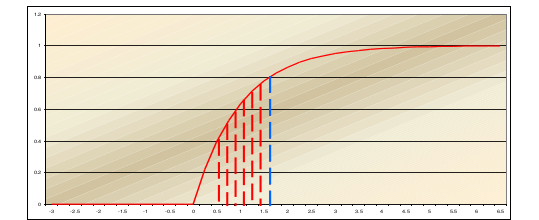
\includegraphics[scale=0.6]{img/con.png}
\end{figure}
Pertanto, quando si pensa a variabili aleatorie continue, non ha mai senso domandarsi quale sia la probabilità
che esse assumano valori esatti, ma conviene invece domandarsi quale è la probabilità che essi assumano
specifici valori appartenenti in specifici intervalli dell'asse reale.

Per calcolare la probabilità che una variabile casuale continua $X$ assuma un valore in un intervallo 
$(a,b] \subseteq \R$ è possibile far ricorso alla formula:
\[ P(X \in (a,b]) = \int _a ^b f_X(u)du\,\,\,  \text{da cui si ricava}\]
\[ \begin{split}
    P(X \in (a, b]) & = F_X(b) - F_X(a) \\
                    & = \int_{-\infty}^b f_X(u)du - \int_{-\infty}^a f_X(u)du\\
   \end{split} \]
In pratica la probabilità che sia soddisfatto l'evento $X\in(a,b]$ corrisponde all'area sottesa
dalla densità $f_X$ nell'intervallo $(a,b]$, come si può notare nella figura ~\ref{graficoRipartizione}, per cui

\begin{figure}
    \center
    \caption{Esempio di calcolo della densità di probabilità continua}
    \label{graficoRipartizione}

    \psscalebox{1.0 1.0} % Change this value to rescale the drawing.
{
\begin{pspicture}(0,-2.375)(8.38,2.375)
\psbezier[linecolor=black, linewidth=0.04](5.9990716,0.4275487)(5.9981446,1.2275481)(1.6000015,-0.37754923)(1.6009284,-1.1775487080233007)
\psline[linecolor=black, linewidth=0.04, arrowsize=0.05291667cm 2.0,arrowlength=1.4,arrowinset=0.0]{->}(0.8,-2.375)(0.8,2.425)
\psline[linecolor=black, linewidth=0.04, arrowsize=0.05291667cm 2.0,arrowlength=1.4,arrowinset=0.0]{->}(0.4,-1.975)(7.2,-1.975)
\psline[linecolor=black, linewidth=0.04, linestyle=dashed, dash=0.17638889cm 0.10583334cm](1.6,-1.175)(1.6,-1.975)
\psline[linecolor=black, linewidth=0.04, linestyle=dashed, dash=0.17638889cm 0.10583334cm](6.0,0.425)(6.0,-1.975)
\rput[bl](1.6,-2.375){$a$}
\rput[bl](5.6,-2.375){$b$}
\rput[bl](7.2,-2.375){$X$}
\rput[bl](-0.1,2.025){$f_X()$}
\rput[bl](6.4,-0.775){$P(X\in(a,b])$}
\psline[linecolor=black, linewidth=0.04, linestyle=dotted, dotsep=0.10583334cm](5.6,0.425)(2.0,-1.175)
\psline[linecolor=black, linewidth=0.04, linestyle=dotted, dotsep=0.10583334cm](5.6,0.025)(2.0,-1.575)
\psline[linecolor=black, linewidth=0.04, linestyle=dotted, dotsep=0.10583334cm](5.6,-0.375)(2.0,-1.975)
\psline[linecolor=black, linewidth=0.04, linestyle=dotted, dotsep=0.10583334cm](5.6,-0.775)(2.8,-1.975)
\psline[linecolor=black, linewidth=0.04, linestyle=dotted, dotsep=0.10583334cm](5.6,-1.175)(3.6,-1.975)
\psline[linecolor=black, linewidth=0.04, linestyle=dotted, dotsep=0.10583334cm](5.6,-1.575)(4.8,-1.975)
\end{pspicture}
}

\end{figure}

\[[P(X\in(a,b]) = \int_a^bf_X(u)du\,\,\,\forall a,b \in \R,\,\,\,a<b\]
Essendo inoltre $P(X = a) = 0$ si ha:
\[ P(X \in (a, b]) = P(X\in[a,b])\,\,\,\forall a,b \in \R,\,\,\,a<b\]
Si ha che la funzione di ripartizione è la funzione integrale della funzione di densità di probabilità,
quindi si ottiene la funzione di densità di probabilità tramite derivazione:
\[\frac{d}{dt} F_X(t) = f_X(t)\]

\subsection{Variabili Aleatorie Multidimensionali}
In molti casi è lecito considerare situazioni (esperimenti) il cui esito è rappresentato, 
anziché da un valore numerico, da una coppia o da una n-pla di valori, in tal caso 
si parla di \textit{variabili aleatorie multidimensionali}.\newline
Anche qui le variabili sono definite da uno spazio campione $\Omega$ a $\R^n$, con $n$ dimensione della variabile,
ed è comodo pensare a queste variabili aleatorie come a risultati esprimibili da n-ple di valori numerici.\newline
Consideriamo quindi le \emph{variabili aleatorie bidimensionali assolutamente continue}, 
anche se ovviamente si può estendere a $n$ variabili anche non continue.

Sia quindi una variabile aleatoria $(X, Y): \Omega \to \R ^ 2$ con $\Omega$, uno spazio campione 
al quale è associata una probabilità $P$ definita sui sottoinsiemi di $\Omega$.\newline
Si definisce la \emph{funzione di ripartizione congiunta} la funzione bidimensionale 
$F_{X, Y}(t, s):\R ^2 \to [0,1] \subseteq \R$ definita come:
\[F_{X, Y} = P(\{X \leq t\} \cap \{Y \leq s\}\,\,\,\forall (t,s)\in \R\]
inoltre se la variabile $(X,Y)$ è assolutamente continua esiste la \emph{funzione dei densità congiunta}
$f_{X, Y}:\R ^2 \to \R_+$ tale che
\[F_{X, Y}(t, s) = \int_{-\infty}^t \int_{-\infty}^s f_{X, Y}(u, v)du\,dv\,\,\,\forall (t, s)\in \R ^2\]
Conoscendo una delle due funzioni sopra è possibile determinare la probabilità che la coppia $(X,Y)$ assuma
valori in un qualsiasi sottoinsieme rettangolare $(a_1, b_1] \times (a_2, b_2] \in \R^2$, in cui risulta:
\[ \begin{split}
    P((X, Y) \in (a_1, b_1] \times (a_2, b_2]) & = F_{X, Y} (b_1, b_2) - F_{X, Y}(a_1, b_2)\\ 
                                               & - F_{X, Y} (b_1, a_2) + F_{X, Y}(a_1, a_2) \\
    & = \int_{a_1}^{b_1} \int_{a_2}^{b_2} f_{X, Y}(u, v) du\,dv\,\,\, \forall (a_1, b_1] \times(a_2, b_2] \in \R^2\\
   \end{split}\]

\begin{figure}
    \caption{Densita di probabilità multidimensionale}
    \label{img:densitaMulti}
    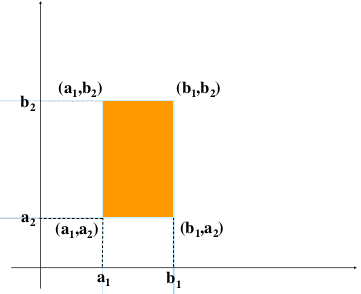
\includegraphics[scale=0.7]{img/mul.png}
\end{figure}
In molti casi, benché ci si trovi di fronte a situazioni i cui esiti sono di tipo multidimensionale, 
capita di essere interessati ai valori che possono essere assunti solamente da una delle variabili per cui 
sono state introdotte le \emph{funzioni marginali}.

Data una variabile aleatoria bidimensionale $(X, Y)$ assolutamente continua, avente 
funzione di ripartizione congiunta $F_{X, Y}$ e funzione di densità disgiunta $f_{X, Y}$ è detta 
\emph{funzione di ripartizione marginale di X} in caso si ha
\[ \begin{split}
    F_X(t) & = P(\{X \leq t\} \cap \{Y \leq +\infty\})\\
           & = F_{X, Y}(t, +\infty)\\
   \end{split}\]
mentre si definisce la funzione p detta \emph{funzione di densità marginale di X} come
\[f_X(t) = \int_{-\infty}^{+\infty} f_{X, Y}(t, s)\,ds\]
Data una variabile bidimensionale $(X, Y)$ diciamo che le due variabili considerate singolarmente 
sono \emph{stocasticamente indipendenti} se e solo se per ogni $(t, s) \in \R^2$ vale
\[F_{X, Y}(t, s) = F_X(t) \cdot F_Y(s)\]
che discende dalla definizione di stocasticamente indipendente fornita nella teoria assiomatica della probabilità.

\section{Indici delle variabili aleatorie}
Iniziamo ad affrontare gli indici associati alle variabili aleatorie, partendo prima dagli indici centrali,
grandezze numeriche associate alle variabili aleatorie, in grado di sintetizzare, con un solo valore,
le principali caratteristiche delle loro distribuzioni.\newline
Gli indici risultano strettamente legati agli indici introdotti nella prima parte in relazione alla 
statistica descrittiva, il più importante degli indici di tendenza centrale è detto \emph{valore atteso}
corrispondente alla media matematica dei dati statistici.

Data una variabile aleatoria unidimensionale $X$ avente supporto $S \subseteq \R$ è detto valore atteso di $X$ la quantità:
\[E[X] = \begin{dcases}
           \sum_{s\in S}\,\, s\cdot p_X(s) \,\,\mbox{ se X è discreta}\\
           \int_{-\infty}^{+\infty}\,\, u\cdot f_X(u)\,du \,\,\mbox{ se X è assolutamente continua}\\
         \end{dcases}\]
In effetti il valore atteso, così come la media di una serie di dati, va pensato come una \textit{media pesata}
dei valori assumibili dalla variabile, e fornisce un'indicazione di massima del posizionamento della variabile
lungo l'asse dei numeri reali.\newline
È possibile volere calcolare il valore atteso da una funzione $g(X)$, anch'essa una variabile aleatoria, per cui esiste
una distribuzione e che è comparabile alla conoscenza della distribuzione di $X$\newline
Questo calcolo effettuato su una funzione $g(X)$ è una generalizzazione della definizione della definizione del valore
atteso effettuato su una variabile $X$ e ciò ci permette di definire e dimostrare una serie di proprietà utili.\newline
La definizione di valore atteso di una funzione $g(X)$ di una variabile aleatoria è la seguente:
\[ E[g(X) = \begin{cases}
                \sum_{x\in S}\,\, g(x)\cdot p_X(x) \,\,\mbox{ se g(X) è discreta}\\
                \int_{-\infty}^{+\infty}\,\, g(x)\cdot f_X(x)\,dx \,\,\mbox{ se g(X)è assolutamente continua}\\
            \end{cases}\]
Il valore atteso gode delle seguenti tre proprietà:
\begin{enumerate}
    \item $\forall a \in \R$, se $X = a$ con probabilità uguale ad 1, allora $E[X] = a$
    \item $E[a\cdot X + b] = a\cdot E[X] + b$ per ogni variabile $X$ e per ogni $a, b \in \R$
\end{enumerate}
\begin{proof}
    Iniziamo a dimostrare $E[aX + b]$ nel caso discreto per poi farlo nel caso continuo
    \[ \begin{split}
        E[aX + b] & = \sum (ax + b) p(x) \\
                  & = \sum ax p(x) + \sum b p(x)\\
                  & = a \sum x p(x) + b \sum p(x) \\
                  & = aE[x] + b\\
       \end{split} \]
    Nel caso continuo avviene lo stesso procedimento, solo che si utilizzano gli integrali invece
    della sommatoria, come si può vedere nella riga successiva.
    \[ \begin{split}
        E[aX + b] & = \int_{-\infty}^{+\infty} (ax + b) f(x) dx \\
                  & = \int_{-\infty}^{+\infty} ax f(x) dx + \int_{-\infty}^{+\infty} b f(x) dx \\
                  & = a \int_{-\infty}^{+\infty} x f(x) dx + b \int_{-\infty}^{+\infty} f(x) dx \\
                  & = aE[X] + b \\
        \end{split} \]
\end{proof}
Il valore atteso non è detto che esista, infatti in caso l'integrale o la sommatoria non convergono il valore
atteso risulta non definito e come avevamo già visto con la media, il valore atteso è in realtà un caso
particolare di momento centrale di ordine $r = 1$, la cui formula è definita come:
\[ E[X^n] = \begin{dcases}
                \sum _x \,\, x^n \cdot p(n) \,\,\mbox{se X è discreta}\\
                \int_{-\infty}^{+\infty}\,\, x^n \cdot f_X(x)\,dx \,\,\mbox{ se X è assolutamente continua}\\
            \end{dcases}\]
Un altro indice di tendenza centrale importante è la \emph{moda} di una variabile aleatoria $X$, indicata
con $\widetilde{X} \in \R$, corrispondente al valore per cui è massima la distribuzione discreta di
probabilità, se $X$ è discreta, oppure rappresenta la funzione di densità; tale valore non è detto che sia
unico, ma può avere la presenza di più valori di moda, e ciò porta a parlare di distribuzione multimodale.

Un terzo indice di tendenza centrale è la \emph{mediana}  di una variabile aleatoria $X$, 
indicata con $\hat{X} \in \R$, che soddisfa la diseguaglianza:
\[ \lim_{t \to \hat{X}^-} F_X(t) \leq \frac{1}{2} \leq F_X(\hat{X})\]
Nel caso in cui la funzione di ripartizione della variabile sia continua ed invertibile allora:
$\hat{X}=F_X^{-1}(\frac{1}{2})$ mentre nel caso di variabili discrete la mediana è il valore dell'ascissa
in cui la funzione di ripartizione passa da un valore minore di $\frac{1}{2}$ ad uno superiore.\newline
La mediana può non essere unica, e ciò avviene in caso esistano più valori $t$ per cui risulta $F_X(t) = \frac{1}{2}$.

\begin{figure}
    \centering
    \caption{grafico di moda, mediana e media}
    \label{fig:centralValue}
    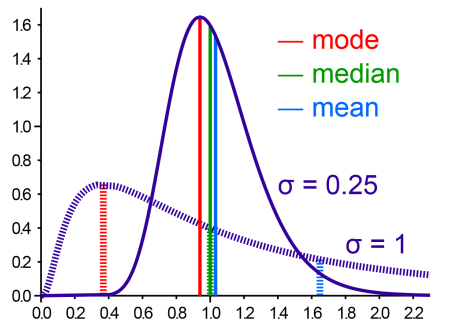
\includegraphics[scale=0.7]{img/mmm.png}
\end{figure}
Unitamente alla mediana è possibile considerare altri indici definiti in maniera simile e che dividono
la retta dei reali in due intervalli di probabilità assegnata e che sono detti \emph{quantili}, come si nota
nella \figurename~\ref{fig:quantile}.
Dato un valore $P \in [0,1] \subseteq \R$ è detto \emph{quantile p-esimo della variabile aleatoria X} il valore
$x_p \in \R$ tale che
\[ \lim_{t \to x_p^{-}} F_X(t) \leq p \leq F_X(x_p)\]
Nel caso in cui la funzione di ripartizione sia continua ed invertibile, allora $x_p = F_X^{-1}(p)$
e questa definizione ci porta a pensare a $x_p$ come ad un valore in cui risulta 
$P(X \leq x_p) = p$ e $P(X > x_p) = 1-p$.

\begin{figure}
    \centering
    \caption{Grafico del quantile}
    \label{fig:quantile}
    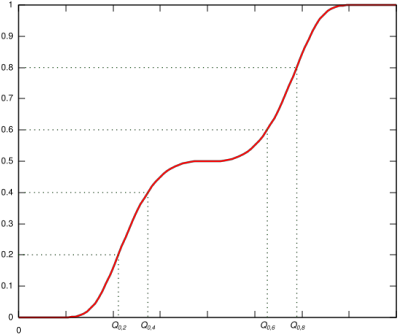
\includegraphics[scale=0.5]{img/qua.png}
\end{figure}

Come visto in precedenza, nella statistica descrittiva, oltre agli indici di tendenza centrale è conveniente 
anche considerare indici che forniscano un'idea del grado di dispersione dei valori 
assumibili da una variabile aleatoria.\newline
Questi vengono detti \emph{indici di variabilità}: il più famoso tra tutti è la \emph{varianza}
di una variabile aleatoria $X$, indicata con $\sigma_X ^ 2$, definita come:
\[V[X] = \begin{dcases}
            \sum_{x}\,\, (x - E[X])^2 \cdot p_X(x)\mbox{ se X è discreta}\\
            \int_{-\infty}^{+\infty}\,\, (x - E[X])^2 \cdot f_X(x)\,dx\mbox{ se X è assolutamente continua}\\
         \end{dcases}\]
Un'altra definizione della varianza, molto utile da calcolare e da usare nelle dimostrazione è la seguente:
\[ \begin{split}
    V[X] & = E[(X - \mu)^2] \\
         & = E[X^2 - 2\mu X + \mu ^2] \\
         & = E[X^2] - 2\mu E[X] + \mu ^2\\
         & = E[X^2] - 2\mu ^2 + \mu ^2 \\
         & = E[X^2] - (E[X])^2\\
    \end{split} \]
Così come il valore atteso anche la varianza talvolta può non esistere, quando la sommatoria o l'integrale divergono.\newline
La radice della varianza è anch'esso un altro indice importante, detto \emph{deviazione standard}, il cui
vantaggio rispetto alla varianza è quello di avere la stessa unità di misura del valore atteso.

Prima di andare a definire le proprietà della varianza, andiamo a definire il valore atteso di 2 variabili come
\[ E[g(X, Y)] = \begin{cases}
                    \sum _y \sum _x g(x, y) p(x, y) \mbox{ se X è discreta} \\
                    \int _{-\infty}^{+\infty} \int _{-\infty}^{+\infty} g(x, y) f(x, y) dx dy \\
                \end{cases} \]
Riguardo al valore atteso di due variabili aleatorie si ha la seguente proprietà:
\begin{teo}
    \[ E[X + Y] = E[X] + E[Y] \]
    \[ E[X_1 + X_2 + \dots + X_n] = \sum _i ^ n E[X_i] \]
\end{teo}
\begin{proof}
    \[ \begin{split}
        E[X + Y] & = \int _{-\infty}^{+\infty} \int _{-\infty}^{+\infty} (x + y) f(x, y) dx dy\\
                 & = \int _{-\infty}^{+\infty} \int _{-\infty}^{+\infty} x f(x, y) dx dy + 
                     \int _{-\infty}^{+\infty} \int _{-\infty}^{+\infty} y f(x, y) dy \\
                 & = E[X] + E[Y] 
        \end{split} \]
    In maniera analoga si dimostra nel caso discreto, in cui si usa ovviamente il simbolo di sommatoria 
    mentre nel caso di somma di 3 o più variabili si applica più volte la somma di 2 variabili, fino ad arrivare 
    a sommare $n$ variabili aleatorie.
\end{proof}
La varianza ha le seguenti proprietà:
\begin{enumerate}
    \item $\forall a \in \R$, se $X = a$ con probabilità uguale ad 1 allora $V[X] = 0$
    \item $V[a\cdot X + b] = a^2 \cdot V[X]$ per ogni variabile $X$ e per ogni $a,b \in \R$
    \item $V[X] = E[X^2] - (E[X])^2\,\,\forall X$ variabile aleatoria
\end{enumerate}
\begin{proof}
    \[ \begin{split}
        V[aX + b] & = E[(aX + b - E[aX + b])^2] \\
                  & = E[(aX + b - aE[X] - b)^2] \\
                  & = E[(aX - a\mu)^2] \\
                  & = a^2 E[(X - \mu)^2] \\
                  & = a^2 V[X]\\
       \end{split} \]
\end{proof}
Nel caso della varianza non è generalmente vero che la varianza della somma di variabili aleatorie concide con la 
somma delle varianze delle singole variabili aleatorie.\newline
In caso le variabili aleatorie sono indipendenti al somma di variabili aleatorie coincide alla somma delle varianze
ma per poterlo dimostrare e definire formalmente dobbiamo prima introdurre il concetto di covarianza.\newline
La covarianza, come già visto nel capitolo sulla statistica descrittiva, ci fornisce il grado di indipendenza di
due o più variabili aleatorie ed è definita con le seguenti due definizioni:
\begin{itemize}
    \item \[ Cov(X, Y) = E[(X - \mu_x) (Y - \mu_y)] \]
    \item \[ \begin{split}
             Cov(X, Y) & = E[(X - \mu_x)(Y - \mu_y)] \\
                       & = E[XY - \mu_yX - \mu_xY + \mu_x\mu_y] \\
                       & = E[XY] -\mu_yE[X] - \mu_xE[Y] + \mu_x\mu_y\\
                       & = E[XY] -\mu_x\mu_y - \mu_x\mu_y + \mu_x\mu_y \\
                       & = E[XY] - E[X]E[Y]\\
            \end{split} \]
\end{itemize}
La covarianza prevede le seguenti proprietà, utile per dimostrazioni e per calcolare le varianze composte:
\begin{itemize}
    \item \[ Cov(aX, Y) = aCov(X, Y) \]
        \begin{proof}
            \[ \begin{split}
                Cov(aX, Y) & = E[(aX - \mu_x)(Y - \mu_y)] \\
                           & = E[aXY - aX\mu_y - \mu_xY + \mu_x\mu_y]\\
                           & = aE[XY] - a\mu_yE[X] - \mu_xE[Y] + \mu_x\mu_y\\
                           & = aE[XY] - a\mu_x\mu_y \\
                           & = a(E[XY] - \mu_x\mu_y \\
                           & = aCov(X, Y)\\
                \end{split} \]
        \end{proof}
    \item \[ Cov(X + Z, Y) = Cov(X, Y) + Cov(Z, Y) \]
          \begin{proof}
              \[ \begin{split}
                  Cov(X + Z, Y) & = E[(X + Z)Y - E[X + Z]E[Y] \\
                                & = E[XY] + E[ZY] - E[X]E[Y] - E[Z]E[Y] \\
                                & = Cov(X, Y) + Cov(Z, Y)\\
                 \end{split} \]
          \end{proof}
    \item \[ Cov(\sum _{i = 1}^n X_i, Y) = \sum _{i = 1}^n Cov(X_i, Y) \]
          \begin{proof}
            Per $n = 2$ il risultato era stato appena dimostrato, per cui proviamo a ripetere lo stesso procedimento per $n = 3$
              \[ \begin{split}
                  Cov(X_1 + X_2 + X_3, Y) & = E[(X_1 + X_2 + X_3)Y - E[X_1 + X_2 + X_3]E[Y]\\
                                          & = E[X_1Y] + E[X_2Y] + E[X_3Y] - E[X_1]E[Y] - E[X_2]E[Y] - E[X_3]E[Y]\\
                                          & = Cov(X_1, Y) + Cov(X_2, Y) + Cov(X_3, Y)\\
                  \end{split} \]
              Applicando lo stesso procedimento per $n > 3$ si ottiene il procedimento appena dimostrato
          \end{proof}
    \item \[ Cov(\sum _{i = 1}^n X_i, \sum_{j = 1} ^m Y_j) = \sum _{i = 1}^n \sum _{j = 1} ^m Cov(X_i, Y_j) \]
          \begin{proof}
              \[ \begin{split}
                  Cov(\sum _{i = 1}^n X_i, \sum_{j = 1} ^m Y_j) 
                        & = \sum _{i = 1}^n Cov(X_i, \sum _{j = 1}^m Y_j) \mbox{ per la proprietà precedente dimostrata}\\
                        & = \sum _{i = 1}^n Cov(\sum _{j = 1}^m Y_j, X_i) \mbox{ per la simmetria della funzione}\\
                        & = \sum _{i = 1}^n \sum _{j = 1}^m Cov(Y_j, X_i \\
                        & = \sum _{i = 1}^n \sum _{j = 1}^m Cov(X_i, Y_j) \mbox{ per la simmetria della covarianza}\\
                  \end{split} \]
          \end{proof}
    \item \[ V[\sum _{i = 1}^n X_i] = \sum _{i = 1}^n V[X_i] + \sum _{i = 1}^n \sum{j = 1, j \neq i}^m Cov(X_i, Y_j) \]
          \begin{proof}
              La dimostrazione deriva dalla proprietà precedentemente dimostrata, impostando $m = n$ e $Y_j = X_j$
              per $j = 1\dots n$
          \end{proof}
    \item \[ V[X + Y] = V[X] + V[Y] + 2Cov(X, Y) \]
          \begin{proof}
              Questo è un corollario del teorema appena dimostrato, ponendo $n = 2$ e sapendo che $Cov(X, Y) = Cov(Y, X)$
          \end{proof}
    \item Date $n$ variabili aleatorie indipendenti $X_1, X_2, \dots, X_n$ si ha che
          \[ V[\sum _{i = 1}^n X_i] = \sum _{i = 1}^n V[X_i] \]
          \begin{proof}
              Partendo dal caso semplice, ossia $n = 2$, sappiamo dal corollario precedente che 
              \[ V[X_1 + X_2] = V[X_1] + V[X_2] + 2Cov(X_1, X_2) \]
              Essendo $X_1$ e $X_2$ indipendenti risulta che $Cov(X_1, X_2) = 0$ e quindi $V[X_1 + X_2] = V[X_1] + V[X_2]$.\newline
              Applicando questo aspetto per le altre $n - 2$ variabili aleatorie indipendenti si verifica la
              proposizione, ossia $V[\sum _{i = 1}^n X_i] = \sum _{i = 1}^n V[X_i]$.
          \end{proof}
\end{itemize}
In caso la covarianza è nulla le due variabili aleatorie vengono dette \emph{incorrelate}, relazione meno 
forte della indipendenza stocastica, come già avevamo notato nel capitolo sulla statistica descrittiva.\newline
Dalla sua definizione si nota che $Cov(X, Y) = Cov(Y, X)$ e che $Cov(X, X) = E[(X - \mu)(X - \mu)] = V[X]$
Anche per le variabili multidimensionali ed in particolare per quelle bidimensionali 
esistono indici di tendenza centrale e variabilità.\newline
Sia $(X, Y)$ una variabile aleatoria bidimensionale discreta o continua, sono detti \emph{valori attesi marginali} 
e \emph{varianza marginali }le quantità $E[X]\,\,E[Y]\,\,V[Y]\,\,V[Y]$
ottenute considerando le distribuzioni marginali di $X$ ed $Y $ ed integrando (o sommando) in accordo ai sistemi visti sopra.

Un ultimo indice è quello detto \emph{coefficiente di correlazione di Pearson}, strettamente legato 
alla covarianza ed utilizzato per esprimere più chiaramente il grado di dipendenza tra due variabili:
\[Corr(X, Y) = \frac{Cov(X,Y)}{\sqrt{V[X]\cdot V[Y]}} = \frac{Cov(X,Y)}{\sigma_x\cdot \sigma_y}\]
questo indice possiede le seguenti proprietà:
\begin{enumerate}
    \item $Corr(XY) = 0$ se $X$ e $Y$ sono incorrelate
    \item $|Corr(XY)| = 1$ se vale la relazione $Y= aX + b\,\,\,\forall a,b \in \R$
\end{enumerate}

La funzione generatrice $\phi(t)$ del momento di una variabile $X$ è definita come
\[ \phi(t) = E[e ^{tX}] = \begin{cases}
                              \sum _x e^{tx} p(x) \mbox{ con $X$ una variabile discreta}\\
                              \int _{-\infty}^{+\infty} e^{tx} f(x) dx \mbox{ con $X$ variabile assolutamente continua}\\
                          \end{cases} \]
La funzione generatrice non è detto che esiste, in quanto il valore atteso $E[e^{tX}]$ potrebbe non esistere, anche se 
nel momento $\phi(0)$ la funzione esiste sempre ed è uguale a $1$.\newline
La funzione generatrice $\phi(t)$ ci fornisce il momento $n$-esimo di una variabile aleatoria $X$, attraverso la
differenzazione della variabile, come si può notare ora nel proseguo
\[ \phi'(t) = \frac{d}{dt} E[e^{tx}] = E[\frac{d}{dt} e^{tx}] = E[xe^{tx}] \]
Calcolando il momento primo rispetto a $0$ otteniamo $\phi'(0) = E[X]$, cosa che sapevamo già dalla statistica descrittiva
mentre similarmente se deriviamo ancora il $\phi'(t)$ otteniamo il momento secondo come segue
\[ \phi''(t) = \frac{d}{dt} \phi'(t) = \frac{d}{dt} E[xe^{tx}] = E[\frac{d}{dt}(xe^{tx})] = E[x^2e^{tx}] \]
Calcolando il momento secondo rispetto a $0$ otteniamo che $\phi''(0) = E[X^2]$ ed in generale risulta
\[ \phi^n(0) = E[X^n] \quad n geq 1 \]
\begin{teo}
    Date due variabili indipendenti $X$ e $Y$ risulta che $\phi_{X + Y}(t) = \phi_X(t) \cdot \phi_Y(t)$
\end{teo}
\begin{proof}
    \[ \begin{split}
        \phi_{X + Y}(t) & = E[e^{t(x + y)} \\
                        & = E[e^{tx} e^{ty}] \\
                        & = E[e^{tx}] E[e^{ty}] \\
                        & = \phi_X(t) \cdot \phi_Y(t) \\
        \end{split} \]
\end{proof}
Un'altro importante aspetto della funzione generatrice è che determina la distribuzione di una variabile, quindi può
essere usata come modo alternativo per definire la funzione di ripartazione di una variabile.

\chapter{Distribuzioni Notevoli}
Essendoci una correlazione, come notato nel precedente capitolo, tra la funzione di ripartizione e
la sua distribuzione/densità di probabilità, si parla di \textbf{distribuzione} di una variabile
intentendo indifferentemente la sua ripartizione o la sua densità/distribuzione.\newline
Con $X \sim F$ si indica che la variabile $X$ è distribuita secondo la distribuzione $F$.

Adesso affrontiamo una serie di distribuzioni famose, che hanno un notevole successo ed utilizzo in campo
statistico e probabilistico, incominciando dalle distribuzioni discrete e poi si analizzano quelle assolutamente continue.

\section{Distribuzioni discrete}
Le distribuzioni discrete maggiormente utilizzate sono le seguenti:
\begin{itemize}
    \item bernoulliana
    \item binomiale
    \item poisson
    \item geometrica
\end{itemize}
Una variabile aleatoria X è detta distribuita secondo una Bernoulliana di parametro $p\in[0,1]$, indicata con
$X \sim B(p)$ se essa può assumere solo i valori 1 e 0 rispettivamente con probabilità $p$ e $(1 - p)$.\newline
Questa distribuzione presenta le seguenti funzioni di ripartizione e la sua corrispondente distribuzione di probabilità:
\begin{itemize}
    \item $p_X(t) = \begin{cases}
                    1 - p \mbox{ se } t = 0\\
                    p     \mbox{ se } t = 1\\
                    0     \mbox{ altrimenti}\\
                    \end{cases}$
    \item $F_X(t) = \begin{cases}
                    0     \mbox{ se } t < 0\\
                    1 - p \mbox{ se } 0 \leq t < 1\\
                    1     \mbox{ se } t \geq 1\\
                    \end{cases}$
\end{itemize}
L'importanza di questa semplice distribuzione è ovvia, in quanto sono variabili di Bernoulli tutte quelle
che individuano il verificarsi di uno specifico evento e che valgono 1 se questo si verifica e 0 altrimenti.

Attraverso l'applicazione della definizione di valore atteso e di varianza si ottiene:
    \[ E[X] = 0 \cdot (1-p) + 1\cdot p = p\]
    \[ V[X] = [0^2 \cdot (1-p) + 1^2 \cdot p] = (1-p) \cdot p\]

Siano $X_1, \cdots, X_n \,  n$ variabili Bernoulliane di identico parametro $p$ e stocasticamente indipendenti tra loro,
e sia anche $X = \sum X_i$, variabile definita distribuita secondo una binomiale di parametri $n$ e $p$,
espressa con $X \sim Bin(n, p)$, se tale variabile può assumere qualsiasi valore intero $k$ compreso tra 0 e $n$,
in accordo con la seguente probabilità:
\[ P(X = k) = \binom{n}{k} \cdot p^k \cdot (1 - p) ^{n-k} \]
La parte $p^k \cdot (1-p)^{n - k}$ fornisce la probabilità che $k$ delle n variabili $X_i$ assumano il valore 1
e che le restanti $n - k$ variabili assumano valore 0 mentre la prima parte $\binom{n}{k}$, come ovvio dal
corso di matematica discreta, fornisce il numero  di combinazioni possibili delle variabili $k$.

In questa distribuzione vengono definite le seguenti funzioni di ripartizione e di distribuzione:
\begin{itemize}
    \item \[p_X(t) = \begin{dcases}
                        \binom{n}{t} p^t (1-p)^{n-t} \mbox{ se } t \in \{0,\cdots, n\}\\
                        0 \mbox{ altrimenti }\\
                     \end{dcases} \]
    \item \[F_X(t) = \sum_{0 \leq k \leq n; k\leq t} \binom{n}{k} p^k (1-p) ^{n - k},\,\,\forall t \in \R\]
\end{itemize}
Le variabili $X_i$ sono indipendenti quindi posso calcolare il valore atteso e la varianza di $X$:
\[E[X] = E[X_1 + \cdots + X_n] = E[X_1] + \cdots + E[X_n] = n \cdot p\]
\[V[X] = V[X_1 + \cdots + X_n] = V[X_1] + \cdots + V[X_n] = n \cdot (1-p) \cdot p\]
La principale applicazione della distribuzione binomiale consiste nella definizione di variabili che "contano" le 
realizzazioni di eventi quando questi siano da considerarsi indipendenti e con identica probabilità di verificarsi.

\begin{figure}
    \caption{Distribuzione binomiale}
    \label{fig:binomiale}
	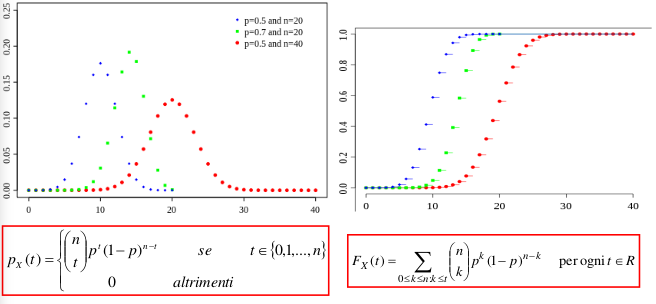
\includegraphics[scale=0.7]{img/dis5.png}
\end{figure}
La distribuzione di Poisson può essere usata per approssimare una Binomiale quando il numero di variabili $X_i$ 
che compaiono in $X = \sum X_i$ tende ad infinito mentre il valore del parametro $p$ tende a zero,
in modo tale che il prodotto $\lambda = n\cdot p$ resti costante.\newline

In caso ciò viene rispettato definiamo $X$ distribuita secondo una Poisson con parametro $\lambda \in \R_+$,
indicata con $X \sim Poi(\lambda)$, applicabile sui valori in $\R$.\newline
La probabilità associata a questa distribuzione è la seguente:
\[ P(X = k) = \lim_{n \to +\infty} \binom{n}{k} \cdot p^k \cdot (1-p)^{n-k} = \frac{\lambda^k}{k!} 
                                                                              e^{-\lambda} \,\, \forall k \in \N\]
la \textit{distribuzione di probabilità} e la \textit{funzione di ripartizione} risultano essere quindi:
\[p_X(t) = \begin{dcases}
           \frac{\lambda^k}{k!} e^{-\lambda} \mbox{ se } t \in \{0,\cdots, n\}\\
           0                                 \mbox{ altrimenti}\\
           \end{dcases}\]
        \[F_X(t) = \sum_{k \in \N:k \leq t} \frac{\lambda^k}{k!} e^{-\lambda},\,\,\forall t \in \R \]
La distribuzione Poisson può essere definita tramite la funzione generatrice $\phi(t)$ come 
\[ \begin{split}
    \phi(t) = E[e^{tx}] & = \sum _{i = 0}^{+\infty} \\
                        & = e^{-\lambda} \sum _{i = 0}^{+\infty} \frac{(\lambda e^t)}{i!} \\
                        & = e^{-\lambda e^{\lambda e^t}} \\
                        & = e^{\lambda(e^t - 1)} \\
    \end{split} \]
Derivando una e due volte la funzione generatrice otteniamo la funzione generatrice prima e seconda
\[ \phi'(t) = \lambda e^t e^{\lambda(e^t - 1)} \]
\[ \phi''(t) = (\lambda e^t)^2 e^{\lambda(e^t - 1)} + \lambda e^t e^{\lambda(e^t - 1)} \]
Valutando a $t = 0$ otteniamo il valore atteso e la varianza come
\[ E[X] = \phi'(0) = \lambda \]
\[ V[X] = \phi''(0) - (E[X])^2 = \lambda^2 + \lambda - \lambda^2 = \lambda \]

La funzione generatrice della somma di variabili poisson indipendenti $X_1$ e $X_2$ è definita come 
\[ \begin{split}
    \phi_{X_1 + X_2}(t) & = E[e^{t(x_1 + x_2)} \\
                        & = E[e^{tx_1} e^{tx_2}]\\
                        & = E[e^{tx_1}] \cdot E[e^{tx_2}]\\
                        & = e^{\lambda_1(e^t - 1)} \cdot e^{\lambda_2(e^t - 1)}\\
                        & = e^{(\lambda_1 + \lambda_2)(e^t - 1)}\\
    \end{split} \]
Essendo la funzione generatrice appena trovata una poisson con $\lambda = \lambda_1 + \lambda_2$ possiamo concludere
che la somma di due variabili poisson indipendenti è anch'essa una poisson, con parametro $\lambda$ uguale alla somma
dei loro parametri $\lambda_1$ e $\lambda_2$.

La distribuzione di Poisson viene utilizzata quando si considerino grandi popolazioni di individui in cui 
ogni individuo ha una probabilità p molto piccola di essere soggetto ad uno specifico evento in esame, come
approssimazione di una binomiale, e per tale ragione la distribuzione di Poisson viene anche detta degli eventi rari.
\begin{figure}
    \caption{Distribuzione di Poisson}
    \label{fig:poisson}
	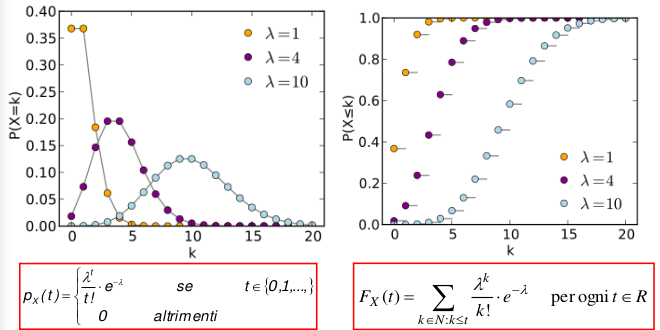
\includegraphics[scale=0.7]{img/dis4.png}
\end{figure}

Una variabile aleatoria X è detta distribuita secondo una Geometrica di parametro $p\in[0,1]$, indicata con $X \sim Geo(p)$,
se può assumere qualsiasi valore intero non negativo k con probabilità $P(X = k) = p \cdot (1-p)^k$.

La distribuzione di probabilità e la funzione di ripartizione risultano essere quindi:
\[p_X(t) = \begin{cases}
            p \cdot (1-p)^t \mbox{ se } t \in \N\\
            0               \mbox{ altrimenti}\\
           \end{cases}\]
\[F_X(t) = \sum_{k \in \N:k \leq t} p \cdot (1-p)^k,\,\,\forall t \in \R\]
con valore atteso e varianza:
\[E[X] = \frac{1-p}{p}\]
\[V[X] = \frac{1-p}{p^2}\]
Questa distribuzione ha la proprietà di \textbf{assenza di memoria}, ossia risulta $P(X = k + m | X \geq m) = P(X = k)$. 

Per comprenderne il significato, supponiamo che X sia il tempo di vita di una macchina soggetta a guasti
, che possono avvenire solo in corrispondenza di intervalli di tempo unitari, e supponiamo di aver rilevato
che per m unità di tempo essa non si sia guastata.\newline
La proprietà di assenza di memoria asserisce che la probabilità che la macchina si guasti all'istante $(k+m)$-esimo,
condizionata dall'evento $X \geq m$, è uguale alla probabilità iniziale che essa si guasti all'istante k-esimo.\newline
Quindi questa proprietà asserisce che il tempo trascorso da quando abbiamo iniziato ad esaminare il funzionamento
della macchina non influisce sulla distribuzione del tempo restante al verificarsi del guasto.

\section{Distribuzioni continue}
Le distribuzioni continue, affrontate in questo corso sono le seguenti:
\begin{itemize}
    \item uniforme
    \item triangolare
    \item esponenziale
    \item normale(o gaussiana)
\end{itemize}
Parliamo ora della \emph{distribuzione uniforme}, che rappresenta la più semplice distribuzione assolutamente continua
e viene adottata nel caso in cui la variabile considerata possa assumere qualsiasi valore compreso
in un dato intervallo con probabilità costante.\newline
Si dice che la variabile $X$ è distribuita secondo una uniforme di supporto $[a,b]$, indicata con $X \sim U[a, b]$
se essa è assolutamente continua con densità e funzione di ripartizione:
\[f_X(t) = \begin{dcases}
            \frac{1}{b-a} \mbox{ se } t \in [a,b]\\
            0             \mbox{ altrimenti}\\
           \end{dcases}\]
\[F_X(t) = \begin{dcases}
            0 \mbox{ se } t < a\\
            \frac{t-a}{b-a} \mbox{ se } t \in [a,b]\\
            1 \mbox{ se } t > b\\
            \end{dcases}\]
            

e con semplici integrazioni è possibile ricavare il valore atteso e la varianza:
\begin{teo}
    \[E[X] = \frac{a+b}{2}\]
    \[V[X] = \frac{(b-a)^2}{12}\]
\end{teo}
\begin{proof}
    \[ \begin{split}
        E[X] & = \int _{\alpha}^{\beta} \frac{x}{\beta - \alpha} dx \\
             & = \frac{\beta^2 - \alpha^2}{2(\beta - \alpha} \\
             & = \frac{(\beta + \alpha)(\beta - \alpha)}{2(\beta - \alpha)}\\
             & = \frac{(\beta + \alpha)}{2}\\
        \end{split} \]
\end{proof}
\begin{proof}
    \[ \begin{split}
        E[X^2] & = \frac{1}{\beta - \alpha} \int _{\alpha}^{\beta} x^2 dx \\
               & = \frac{\beta^3 - \alpha^3}{3(\beta - \alpha)} \\
               & = \frac{\beta^2 + \alpha\beta + \alpha^2}{3}\\
        \end{split} \]
        Sfruttando il fatto appena dimostrato si dimostra che
    \[ \begin{split}
        V[X] & = E[X^2] - (E[X])^2 \\
             & = \frac{\beta^2 + \alpha\beta + \alpha^2}{3} - (\frac{\beta - \alpha}{2})^2\\
             & = \frac{\beta^2 + \alpha^2 - 2\alpha\beta}{12} \\
             & = \frac{(\beta - \alpha)^2}{12} \\
       \end{split} \]
\end{proof}

Come accennato in precedenza l'interesse in questa distribuzione è giustificato dal fatto che essa descrive bene
situazioni nelle quali le variabili possono assumere valori in intervalli finiti di $\R$ con probabilità uniforme,
ovvero tale da essere identica per intervalli di medesima ampiezza, purchè contenuti nel supporto della variabile stessa.
\begin{figure}
    \caption{Distribuzione Uniforme}
    \label{img:uniforme}
	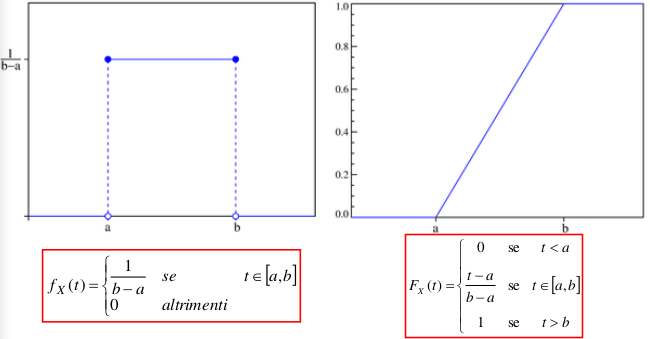
\includegraphics[scale=0.7]{img/dis2.png}
\end{figure}

Ovviamente non è certo che i valori assumibili abbiano tutti la stessa probabilità di presentarsi, per questo
sono stati introdotti alcune generalizzazioni della distribuzione uniforme;una di queste è la
\textbf{distribuzione triangolare}, che assegna alla densità di probabilità valori maggiori al centro del
supporto e minori in prossimità degli estremi.\newline
Formalmente diciamo che la variabile $X$ è distribuita secondo una Triangolare di supporto $[a,b]$, indicata
con $X \sim T[a, b]$ se essa è assolutamente continua con le seguenti funzioni di densità e ripartizione:
\[f_X(t) = \begin{dcases}
            \frac{4(t-a)}{(b-a)^2} \mbox{ se } t \in \left[a,\frac{a+b}{2}\right)\\
            \frac{4(b-t)}{(b-a)^2} \mbox{ se } t \in \left[\frac{a+b}{2},b\right]\\
            0                      \mbox{ altrimenti}
            \end{dcases}\]
\[F_X(t) = \begin{dcases}
            0 \mbox{ se } t<a\\
            \frac{2(t-a)^2}{(b-a)^2} \mbox{ se } t \in \left[a, \frac{a+b}{2}\right)\\
            1-2\frac{(b-t)^2}{(b-a)^2} \mbox{ se } t \in \left[\frac{a+b}{2}, b\right]\\
            1 \mbox{ se } t>b\\
            \end{dcases}\]
Attraverso l'integrazione delle funzioni presentate si ottiene il valore atteso e la varianza:
\[E[X] = \frac{a+b}{2}\]
\[V[X] = \frac{(b-a)^2}{24}\]

Passiamo alla \textbf{distribuzione esponenziale}, importante nello studio di variabili che descrivono i tempi
necessari per il verificarsi di un evento.\newline
Formalmente, una variabile aleatoria $X$ è distribuita secondo una Esponenziale di parametro $\lambda \in \R$,
indicata con $X \sim Exp(\lambda)$ se essa è assolutamente continua con le seguenti funzioni:
\[f_X(t) = \begin{dcases}
            \lambda e^{-\lambda t} \mbox{ se } t \geq 0\\
            0 \mbox{ altrimenti}
            \end{dcases}\]
\[F_X(t) = \begin{dcases}
            1 - e^{-\lambda t} \mbox{ se } t \geq 0\\
            0 \mbox{ altrimenti}
            \end{dcases}\]
La distribuzione esponenziale può essere definita mediante la funzione generatrice come segue
\[ \begin{split}
    \phi(t) & = E[e^{tx}] \\
            & = \int _0 ^{+\infty} e^{tx} \lambda e^{-\lambda x} dx\\
            & = \lambda \int _0 ^{+\infty} e^{-(\lambda - t)x} dx\\
            & = \frac{\lambda}{\lambda - t} \mbox{ con $t < \lambda$}
    \end{split} \]
Derivando una e due volte otteniamo la derivata prima e la derivata seconda
\[ \phi'(t) = \frac{\lambda}{(\lambda - t)^2} \]
\[ \phi''(t) = \frac{2\lambda}{(\lambda - t)^3} \]
Calcolando il momento nel punto $t = 0$ siamo in grado di trovare la varianza e il valore atteso 
\[E[X] = \phi'(0) = \frac{1}{\lambda}\]
\[V[X] = \phi''(0) - (\phi'(0))^2 = \frac{2}{\lambda^2} - \frac{1}{\lambda^2} = \frac{1}{\lambda^2} \]
L'importanza della distribuzione esponenziale in numerosi campi applicativi è dovuta al fatto che essa è
l’unica distribuzione assolutamente continua che gode della \textbf{proprietà di assenza di memoria}, vista
anche nella distribuzione geometrica, di tipo discreto.

\begin{teo}
    Siano $X_1, X_2, \dots, X_n$ delle variabili aleatorie indipendenti esponenziali, aventi parametri $\lambda_1,
    \dots, \lambda_n$, allora $min(X_1, X_2, \dots, X_n)$ è un esponenziale con parametri $\sum _{i = 1}^n \lambda_i$
\end{teo}
\begin{proof}
    Dato che il minor valore di una serie di numeri è più grande di $X$ se e solo se tutti i suoi valori sono più grandi
    di $X$ abbiamo che
    \[ \begin{split}
        P(min(X_1, X_2, \dots, X_n) > X) & = P(X_1 > X, X_2 > X, \dots, X_n > X)\\
                                         & = \prod _{i = 1}^n P(X_i > X) \mbox{ per l'indipendenza}\\
                                         & = \prod _{i = 1}^n e^{-\lambda_i x} \\
                                         & = e^{-\sum _{i = 1}^n \lambda_i x} \\
        \end{split} \]
\end{proof}
\begin{figure}
    \caption{Distribuzione esponenziale}
	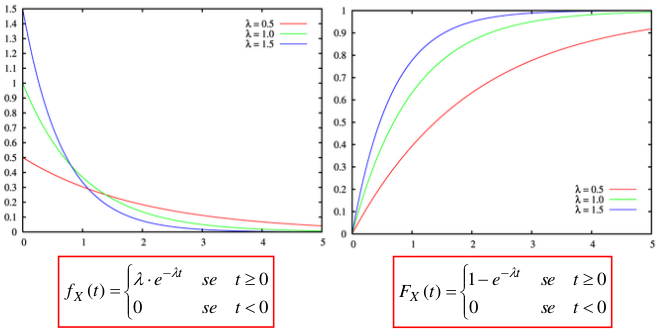
\includegraphics[scale=0.7]{img/dis.png}
\end{figure}
\subsection{Distribuzione Normale}
Una variabile aleatoria X è detta distribuita secondo una \emph{Normale} con parametri $\mu \in \R$ e $\sigma \in \R_+$,
indicata attraverso $X \sim N(\mu, \sigma)$, se essa è assolutamente continua con densità:
\[f_X(x)=\frac{1}{\sqrt{2\cdot \pi\cdot \sigma^2}}\cdot e^{-\frac{(t-\mu)^2}{2\cdot \sigma^2}}\,\,\,\forall t\in\R\]
La funzione di densità di $f_X(x)$ è una curva simmetrica rispetto a $\mu$ e avente come massimo 
$\frac{1}{\sigma \cdots \sqrt{2 \pi}} =  \frac{399}{n \sigma}$ con $x = \mu$.\newline
Questa distribuzione è fondamentale per il \emph{teorema centrale del limite}, studiata nel prossimo
capitolo e poi perchè molti fenomeni studiati dalla statistica e dalla probabilità si comportano come una
normale, chiamata anche \emph{gaussiana} infatti una normale viene usata per approssimare una binomiale, con $n$ grande.

La funzione generatrice momento di una normale è definita come, ponendo $y = \frac{x - \mu}{\sigma}$,
\[ \begin{split}
    \phi(t) & = E[e^{tx}] \\
            & = \frac{1}{\sqrt{2 \pi \sigma}} \int _{-\infty}^{+\infty} e^{tx} e^{-\frac{(x - \mu)^2}{2\sigma^2}} dx \\
            & = \frac{1}{\sqrt{2 \pi}} e^{\mu t} \int _{-\infty}^{+\infty} e^{t \sigma y} e^{\frac{-y^2}{2}} dy \\ 
            & = \frac{e^{\mu t}}{\sqrt{2 \pi}} \int _{-\infty}^{+\infty} e^{\frac{-y^2 - 2t \sigma y}{2}} dy \\
            & = e^{\frac{\mu t + \sigma^2 t^2}{2}} \frac{1}{\sqrt{2\pi}} \int _{-\infty}^{+\infty} e^{\frac{-(y -t\sigma)^2}{2}} dy\\
            & = e^{\frac{\mu t + \sigma^2 t^2}{2}}\\
    \end{split} \]
L'ultimo passaggio deriva dalla definizione di normale, con parametri $t\mu$ e $1$ 
e derivando una e due volte si ottiene 
\[ \phi'(t) = (\mu + t\sigma^2) e^{\mu t + \frac{\sigma^2t^2}{2}} \]
\[ \phi''(t) = \sigma^2 e^{\mu t + \frac{\sigma^2 t^2}{2}} + e^{\mu t + \frac{\sigma^2 t^2}{2}} (\mu + t\sigma^2) \]
Dalle funzioni momento appena calcolate otteniamo il valore atteso e la varianza come
\[E[X] = \phi'(0) = \mu e^0 + 0 = \mu \]
\[V[X] = \phi''(0) - (\phi'(0))^2 = \sigma^2 + \mu^2 - \mu^2 = \sigma^2 \]

\begin{figure}
    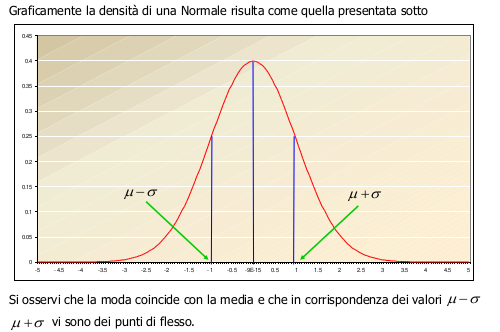
\includegraphics[scale=0.7]{img/norm.png}
\end{figure}
\begin{figure}
    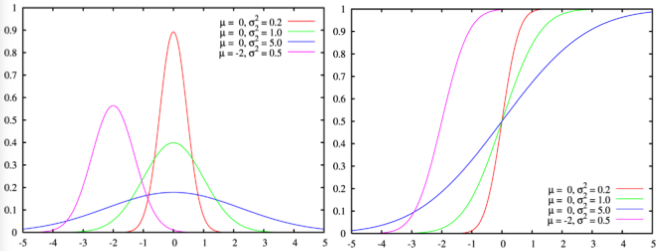
\includegraphics[scale=0.7]{img/nomr2.png}
\end{figure}
Calcolare la probabilità P, assunta da una variabile $X$ in un intervallo $[a, b]$ è notevolmente difficile in
quanto si deve risolvere la seguente equazione:
\[P(X \in [a,b]) = \int_a^b \frac{1}{\sqrt{2\cdot \pi\cdot \sigma^2}}\cdot e^{-\frac{(t-\mu)^2}{2\cdot \sigma^2}}\,dt\]
Per questa ragione si ricorre ad opportune tavole che si riferiscono alla distribuzione normale standard 
ovvero con parametri $\mu = 0$ e $\sigma = 1$ e che forniscono i valori di $\int_0^z f_X(t)\,dt$ 
per un elevato numero di valori $z \in \R$.\newline
Quando si sia interessati a determinare delle probabilità associate ad una generica normale ci si riconduce al
caso sopra osservando che la variabilie $Z = \frac{X - \mu}{\sigma}$ è distribuita secondo una \emph{Normale Standard}
\[\mbox{se } X \sim N(\mu, \sigma) \mbox{ allora } Z = \frac{X \mu}{\sigma} \sim N(0,1)\]
quindi ogni variabile $X \sim N(\mu, \sigma)$ può essere ricondotta ad una può essere ricondotta ad una Normale
standarizzata ovvero ancora per ogni ovvero ancora $\forall [a,b] \subseteq \R$ si avrà:
\[P(X \in [a,b]) = P(a \leq X \leq b) =P \left(\frac{a - \mu}{\sigma} \leq \frac{X-\mu}{\sigma} \leq 
                   \frac{b-\mu}{\sigma}\right) = P \left(Z \in \left[\frac{a-\mu}{\sigma},\frac{b-\mu}{\sigma}\right]\right)\]

La distribuzione gaussiana possiede la seguente proprietà:
\begin{definizione}
     $\mbox{se } X_1 \sim N(\mu_1,\sigma_1) \mbox{ e } X_2 \sim N(\mu_2, \sigma_2)$ e se $X_1$ e $X_2$
        sono indipendenti allora la variabile $Y = X_1 + X_2$ tale che:
        \[Y \sim N(\mu_1 + \mu_2, \sqrt{\sigma_1^2 + \sigma_2^2})\]
\end{definizione}
In altri termini la variabile somma di due variabili aleatorie stocasticamente indipendenti con distribuzioni normali
è ancora una variabile aleatoria distribuita secondo una normale i cui parametri sono ricavabili facilmente
da quelli delle distribuzioni degli addendi.
\begin{shaded}
\subsubsection{La tabella della z}
una volta ottenuto $P\left(Z\in\left[\frac{a-\mu}{\sigma},\frac{a-\mu}{\sigma}\right]\right)$ poniamo per semplicità $\gamma= \frac{a-\mu}{\sigma}$ e $\delta=\frac{b-\mu}{\sigma}$. Per simmetria notiamo che è indifferente valutare $\gamma$ e $\delta$ sia che siano positivi che negativi e per comodità la tabella presenta unicamente valori positivi. Valutemo quindi $|\gamma|$ e $|\delta|$. Sappiamo che $P(Z\in[\gamma,\delta])=P(Z\in[0, |\gamma|])+P(Z\in[0,|\delta|])$. Per calcolare, per esempio, $P(Z\in[0, |\gamma|])$ prendo la cifra intera e la prima cifra decimale e trovo la riga corrispondente nella prima colonna (se $\gamma=1.35$ cercherò $1.3$) e poi cerco scelgo la colonna corrispondente al valore della seconda cifra decimale presente nella prima riga (nel caso di prima cerco nella prima riga il valore $0.05$ e ne scelgo la colonna). L'incrocio fra la riga scelta prima e la colonna scelta dopo mi daranno il valore ricercato. Ecco un esempio con 0.08 e 1.35:
\begin{center}
	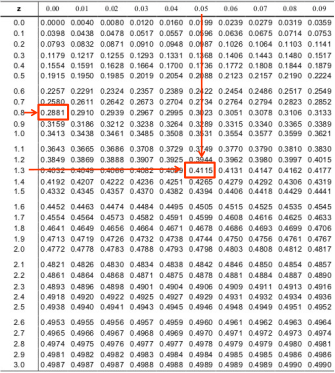
\includegraphics[scale=0.68]{img/z2.png}
\end{center}
\end{shaded}
\begin{shaded}
Regole di calcolo per normali standardizzati da tabelle per integrali:
\begin{itemize}
	\item integrali della forma $\int_{-\infty}^bf(u)\,du$:
	\begin{itemize}
		\item $b>0$, finito:
			\[\int_{-\infty}^b f(u)\, du= \frac{1}{2}+\int_0^b f(u)\, du\]
		\item $b<0$, finito:
			\[\int_{-\infty}^b f(u)\, du= \frac{1}{2}-\int_0^{-b} f(u)\, du\]
	\end{itemize}
	\item integrali della forma $\int_{a}^{+\infty}f(u)\,du$:
		\[\int_{a}^{+\infty}f(u)\,du= 1-\int_{-\infty}^{a} f(u)\, du\]
	\item integrali della forma $\int_{a}^{b}f(u)\,du$:
		\[\int_{a}^{b}f(u)\,du=\int_{-\infty}^bf(u)\,du-\int_{-\infty}^a f(u)\,du\]
\end{itemize}
\end{shaded}
Data una normale di parametri $\mu$ e $\sigma^2$ abbiamo che $Y = \alpha X + \beta$ è una normale, con media $\alpha \mu + \beta$
e varianza $\alpha^2 \sigma^2$ e ciò si dimostra attraverso la funzione generatrice
\[ \begin{split}
    E[e^{t(\alpha X + \beta)} & = e^{t \beta} E[e^{\alpha tX}] \\
                              & = e^{t \beta} e^{\mu \alpha t + \frac{\sigma^2(\alpha t)^2}{2}}\\
                              & = e^{\beta + \mu \alpha)t + \frac{\alpha^2 \sigma^2 t^2}{2}}\\
    \end{split} \]
Da questo segue che se $X \sim N(\mu, \sigma^2)$ allora $Z = \frac{X - \mu}{\sigma}$ è una normale standard, 
con media $0$ e varianza $1$ che ci permette di essere calcolato tramite delle tavole standard di $Z$, 
dato che calcolare la funzione di ripartizione di una normale non è semplice nè immediato.

La somma di variabili normali indipendenti è anch'essa una normale, come mostriamo ora con il seguente teorema
\begin{teo}
    Supponiamo che $X_i$, con $i = 1 \dots n$, siano variabili normali indipendenti, con media $\mu_i$ e varianza $\sigma_i^2$,
    abbiamo che $\sum _{i = 1}^n X_i \sim N(\sum _{i = 1}^n \mu_i, \sum _{i = 1}^n \sigma_i^2)$
\end{teo}
\begin{proof}
    la funzione generatrice di $\sum _{i = 1} ^ n X_i$ è la seguente
    \[ \begin{split}
        E[e^{t \sum_{i = 1}^n X_i}] & = E[e^{tx_1} e^{tx_2} \dots e^{tx_n}] \\
                                    & = \prod _{i = 1}^n E[e^{tx_i}] \mbox{ per l'indipendenza delle variabili}\\
                                    & = \prod _{i = 1}^n e^{\mu_i t + \frac{\sigma_i^2 t^2}{2}} \\
                                    & = e^{\mu t + \frac{\sigma^2 t^2}{2}}\\
       \end{split} \]
    Avendo $\sum _{i = 1}^n X_i$ la stessa funzione generatrice di una normale possiamo concludere che 
    $\sum X_i \sim N(\sum _{i = 1}^n \mu_i, \sum _{i = 1}^n \sigma_i^2)$
\end{proof}
Dopo aver considerato le distribuzioni principali continue, consideriamo 3 distribuzioni utili per la statistica inferenziale:
\begin{itemize}
    \item \textbf{chi-quadro}: siano $X_1, \cdots, X_n n$ variabili con distribuzione normale standard ed
        indipendenti tra loro e sia $X$ una variabile aleatoria definita come 
        \[ X = \sum X_i ^ 2 \]
        si dice distribuita secondo una chi-quadro con n gradi di liberta, indicata con $X \sim \chi_n^2$,
        che ovviamente essendo definita come somma di quadrati può assumere solo valori non negativi.
        
\begin{teo}
        Se $X_1$ e $X_2$ sono 2 variabili chi-quadro, con $n_1$ e $n_2$ gradi di libertà, allora 
        $X_1 + X_2$ è una chi-quadro con $n_1 + n_2$ gradi di libertà.\newline
\end{teo}
\begin{proof}
        Questa proprietà si può facilmente dimostrare dalla definizione di chi-quadro, ponendo $X = X_1 + X_2$,
        e a loro volta sostituire $X_1$ e $X_2$ con la loro definizione, risultando la somma di $n_1 + n_2$ variabili
        normali elevate al quadrato, da cui segue che è chi-quadro con $n_1 + n_2$ gradi di libertà.
\end{proof}
        Se $X$ è una variabile chi-quadro con $n$ gradi di libertà, allora $\forall \alpha \in (0, 1)$ la quantità
        $\chi_{\alpha, n}^2$ è definita come $P(X \geq \chi_{\alpha, n}^2) = \alpha$
        Per calcolare la $\chi$ si usano delle tavole standard che mostrano $\chi^2_{\alpha, n}$, per una certa
        varietà di $\alpha$ e $n$.
    \begin{figure}
            \caption{Distrubuzione chi-quadro}
	        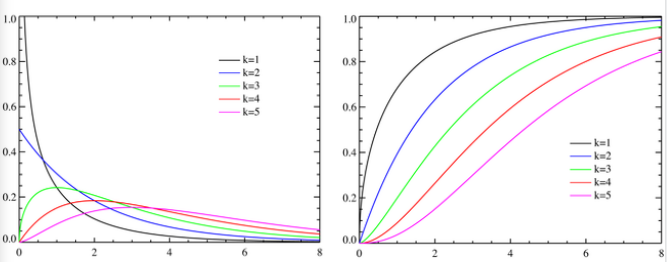
\includegraphics[scale=0.7]{img/chi.png}
        \end{figure}
    \item \textbf{t di student}: siano $Z \sim N(0, 1)$ e $Y \sim \chi_n^2$ due variabili indipendenti e
        sia $X$ una variabile aleatoria definita come 
        \[X = \frac{Z}{\sqrt{\frac{Y}{n}}}\]
        si dice distribuita secondo una t di student con n gradi di libertà, indicata con $X \sim t_n$.

        Come la normale standard, come si può notare nella \figurename~\ref{img:student}, anche la densità di $t$
        è simmetrica a $0$ e in aggiunta con $n$ grande la sua densità diviene molto simile alla densità di una 
        normale standard, per la legge dei grandi numeri, dato che $E[\chi^2]$ converge a $n$, essendo le variabili
        formanti la chi-quadro convergono a $1$ da cui segue che la $t$ può essere approssimata dalla variabile $Z$,
        variabile aleatoria normale standard.
        
        La distribuzione t possiede i seguenti valori atteso e varianza
        \[ E[T_n] = 0 \quad n > 1 \]
        \[ V[T_n] = \frac{n}{n - 2} \quad n > 2 \]
        Anche la distribuzione $t$ viene calcolata mediante le tavole standard, che ci forniscono molti
        valori di $t_{\alpha, n}$ per dei selezionati $\alpha$ e $n$.
        \begin{figure}
            \caption{Distribuzione t di student}
            \label{img:student}
	        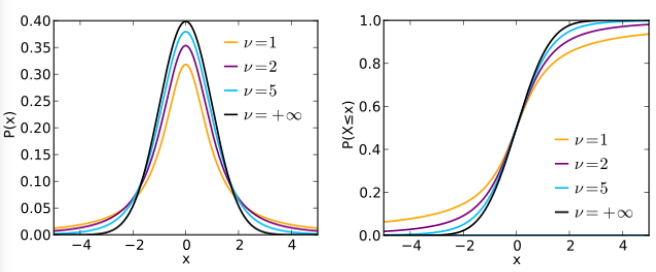
\includegraphics[scale=0.7]{img/t.png}
        \end{figure}

    \item \textbf{distrubuzione f}: siano $U \sim \chi_m^2$ e $V \sim \chi_n^2$ due variabili indipendenti, si
        ha che $X$ una variabile aleatoria definita come 
        \[X = \frac{\frac{U}{n}}{\frac{V}{m}}\]
        si dice distribuita secondo una $F$ con m e n gradi di libertà, indicata con $X \sim F(n, m)$.

        Anche la distribuzione $f$ viene calcolata mediante le tavole standard con $\alpha \leq \frac{1}{2}$,
        sfruttando il fatto che 
        \[ P(F_{n, m} > F_{\alpha, n, m}) = \alpha \]
        In caso $\alpha > \frac{1}{2}$ si può risolvere andando a calcolare
        \[ P(F_{n, m} \geq \frac{1}{F_{\alpha, n, m}}) = 1 - \alpha \]
        \begin{figure}
	        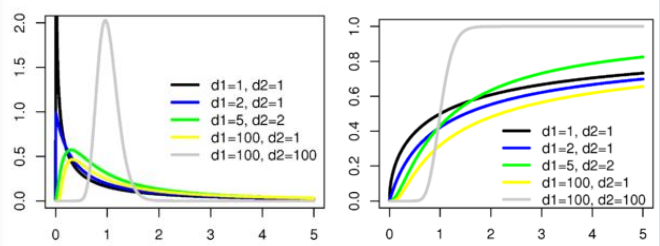
\includegraphics[scale=0.7]{img/f.png}
        \end{figure}
\end{itemize}

\chapter{Teoremi di Convergenza}
Consideriamo una successione $\{X_n, n \in \N\}$ di variabili aleatorie e sia $F_n$ la funzione di ripartizione
della generica variabile $X_n$ della successione.\newline
Diremo che la successione converge in distribuzione alla variabile $X$ avente funzione di ripartizione $F$ se vale:
\[\lim_{n\to\infty} F_n(t) = F(t)\]
per ogni $t \in \R$, punto di continuità per la funzione di ripartizione $F$. 

Si useranno le seguenti notazioni:
\[X_n\stackrel{d}{\longrightarrow} X\]
\[F_n\stackrel{d}{\longrightarrow} F\]
Nella definizione di convergenza in distribuzione vengono esclusi, nel passaggio al limite, i punti 
in cui la funzione di ripartizione limite $F$ è discontinua, per avere un concetto di convergenza simile all'intuizione.

Consideriamo ad esempio una successione di numeri reali $\{a_n, n \in \N\}$ tale che:
\[a_n \stackrel{d}{\longrightarrow} a \in \R \mbox{ per } n \to \infty\]
e pensiamo alle variabili aleatorie $X_n$ aventi funzione di ripartizione:
\[F_n(t) = \begin{cases}
            0 \mbox{ se } t < a_n\\
            1 \mbox{ se } t \geq a_n\\
           \end{cases}\]
ovvero la generica variabile $X_n$ assume valore $a_n$ con probabilità 1.\newline
Da un punto di vista intuitivo siamo portati a pensare che valga $X_n \stackrel{d}{\longrightarrow} X$,
con $X$ avente la funzione di ripartizione:
\[ F(t) = \begin{cases}
            0 \mbox{ se } t < a\\
            1 \mbox{ se } t \geq a\\
          \end{cases}\]
ovvero $X = a$ con probabilità uguale a uno ma la successione $\{a_n, n \in N\}$ tale che:
\[\begin{cases}
        a<a_n\mbox{ con n pari}\\
        a_n<a\mbox{ con n dispari}
  \end{cases}\]
risulta quindi:
\[\begin{cases}
    F_n(a) = 0 \mbox{ per n pari}\\
    F_n(a) = 1 \mbox{ per n dispari}
\end{cases}\]
il limite $\lim_{n \to \infty} F_n(a)$ non esiste quindi è scorretto dire che la successione converge
in distribuzione in quanto non è definibile in $a$ la funzione ripartizione limite $F$;
per evitare questi problemi si esclude, nella definizione di convergenza, i valori in cui la $F$ limite non è continua.

Segnaliamo che la convergenza in distribuzione non è l’unico tipo di convergenza tra variabili aleatorie
definito in letteratura, come ad esempio sono importanti convergenza quasi certa e in probabilità ma
in questo corso di statistica e probabilità abbiamo deciso di non considerarle, in quanto esula dagli scopi
e finalità del nostro corso.

\section{Legge dei Grandi Numeri}
Considero la successione $\{X_i \in \N_+\}$ di variabili aleatorie indipendenti ed identicamente distribuite e
considero poi la variabile aleatoria, detta \emph{media aritmetica n-esima della successione}
\[ \overline{X}_n = \frac{X_1 + \cdots + X_n}{n}\]

Avendo $E[X_i] = \mu$ e $V[X_i] = \sigma^2$, si ha allora $\overline{X}_n \stackrel{d}{\longrightarrow} M$,
con $M$ variabile aleatoria che assume il valore $\mu$ con probabilità 1.\newline
La proprietà appena introdotta costituisce una forma debole del risultato, noto con il nome di \emph{Legge dei Grandi Numeri}.

Nel dettaglio questa legge asserisce che:
\begin{teo}
Se considero una successioni di variabili aleatorie indipendenti ed identicamente distribuite $\{X_i, i \in \N_+\}$
per cui esistono finiti valore atteso e varianza allora si può affermare che la successione:
\[\{\overline{X}_n, n \in \N_+\}\]
delle corrispondenti medie aritmetiche tende, al crescere di $n$, ad una variabile che assume certamente il valore:
\[E[X_i]=\mu\]
\end{teo}
Quindi se considero una successione $\{x_i, i \in \N_+\}$ di realizzazioni delle variabili $\{X_i, i \in \N_+\}$
e considero la successione $\{\overline{x}, n \in \N_+\}$ delle corrispondenti realizzazioni delle medie aritmetiche,
abbiamo che questa seconda successione tende, per n tendente ad infinito, al valore $E[X_i] = \mu$.

Nella realtà le ipotesi della legge dei grandi numeri possono essere indebolite rispetto a quelle definite da
noi, infatti esistono versioni alternative in cui non è richiesta l'ipotesi che le variabili $X_i$ siano
identificamente distribuite.

La legge dei grandi numeri assicura la convergenza $\overline{X}_n \stackrel{d}{\longrightarrow} M$ ma non ci
fornisce alcuna informazione riguardo la rapidità con cui ciò avviene, infatti non sappiamo per quale $n$ è
lecito supporre che la realizzazione $\overline{x}_n$ assuma valore $\mu$ o prossimo ad esso.\newline
È intuitivo pensare che la convergenza avvenga con maggiore rapidità in caso di una varianza molto piccola, e
questo è il \emph{teorema del limite centrale}, in cui viene specificata quale sia la distribuzione della
variabile aleatoria $\overline{X}_n$, con $n$ sufficientemente grande, e quali siano il valore atteso e la
varianza della stessa.

Sia $\{X_i,\in\N_+\}$ una successione di variabili aleatorie che soddisfa le ipotesi della Legge dei Grandi
Numeri, ovvero siano le $X_i$ indipendenti ed identicamente Distribuite ed aventi valore atteso $\mu$ e 
varianza $\sigma^2$, entrambi esistenti e finiti.\newline
Si consideri ora la variabile aleatoria $S_n$, $S_n = \sum X_i$, in cui vale:
\[S_n \stackrel{d}{\longrightarrow} X \sim N(n \cdot \mu, \sqrt{n} \cdot \sigma) = N(n \cdot \mu, n \cdot \sigma^2)\].
Ovvero $S_n$ converge in distribuzione ad una variabile distribuita come una normale di media $n \cdot \mu$ e
deviazione standard $\sqrt{n} \cdot \sigma$.

Osservato che vale $\overline{X}_n = \frac{S_n}{n}$ dalla formula:
\[S_n \stackrel{d}{\longrightarrow} X \sim N(n \cdot \mu, \sqrt{n} \cdot \sigma) = N(n \cdot \mu, n \cdot \sigma^2)\]
si ha che $E[a \cdot X + b] = a \cdot E[X] + b,\,\, \forall X,\,\, \forall a,b \in \R$ e quindi:
\[E[\overline{X}_n] = E\left[\frac{S_n}{n}\right] = \frac{1}{n}E[S_n] = \frac{1}{n} E[X_1+\cdots +X_n] = \frac{1}{n}(n\mu) = \mu\]
inoltre si ha che $V[a \cdot X + b] = a^2 \cdot V[x],\,\, \forall X \,\, \forall a,b \in \R$ e quindi
\[V[\overline{X}_n]=V\left[\frac{S_n}{n}\right]=\frac{1}{n^2}V[S_n]=\frac{1}{n^2}V[X_1+\cdots+X_n]=\frac{1}{n^2}(n\sigma^2)=\frac{\sigma^2}{n}\]
quindi si conclude che:
\[S_n\stackrel{d}{\longrightarrow}X\sim N(\mu, \frac{\sigma}{\sqrt{n}})=N(\mu, \frac{\sigma^2}{n})\]
quindi per $n$ sufficientemente grande possiamo approssimare le variabili $S_n$ e $\overline{X}_n$ con 
delle variabili aventi distribuzione normale i cui parametri dipendono da quelli delle variabili $X_i$.\newline
Si ha inoltre la seguente approssimazione:\\
\textit{n è ritenuto sufficientemente grande sse $n\geq 30$}

\chapter{Stime di Parametri}
La \emph{statistica inferenziale} ci consente di dedurre particolari caratteristice di una popolazione, considerando
ed analizzando un campione finito e preferibilmente piccolo di suoi individui.\newline
In caso si ha caratteristiche esprimibili numericamente si parla di \emph{parametri}, mentre per stima di parametri
si intende il problema della deduzione di caratteristiche di tipo numerico di una popolazione, attraverso
l'analisi di un suo campione oppurtunamente scelto, in maniera casuale.\newline
Per \emph{campionamento casuale} si intende un campione, in cui si assegna la stessa probabilità di essere estratto
ad ogni individuo della popolazione.

Per generare un campione casuale si assegna, in maniera progressiva, un numero ad ogni individuo della popolazione 
e poi si estrae, tramite un qualsiasi generatore casuale, tanti numeri quanti devono essere gli elementi del campione;
questa procedura è dispensiosa dal punto di vista temporale ma è necessaria, dato che ci assicura di avere un
campione casuale, i cui elementi sono stati scelti senza alcun discriminazione e/o considerazione.\newline

Un’altra considerazione che occorre sempre fare durante un’operazione di
campionamento riguarda la possibilità di estrarre più volte uno stesso individuo,
detto \textit{campionamento con ripetizione o senza ripetizione}.\\
La scelta tra queste due alternative diviene rilevante quando la popolazione
considerata è di numerosità limitata e diviene trascurabile nel caso di popolazioni di
vaste dimensioni o infinite e questo è il caso che verrà trattato d’ora in avanti.

Le tecniche per effettuare la stima di parametri sono basate sulla conoscenza delle \emph{distribuzioni campionarie}, 
vale a dire distribuzioni di particolari indici statistici associati alle caratteristiche del campione.

Denotiamo con $X$ il carattere della popolazione considerato, il cui valore assunnto varia a seconda 
dell'individuo considerato, per cui conviene pensare ad X come ad una variabile aleatoria, la cui distribuzione,
sconosciuta, corrisponde a quella che si otterrebbe facendo ricorso alle tecniche di statistica descrittiva.\newline
Si considera per cui i valori assunti dai singoli individui come a delle realizzazioni di X e formalmente un campione
casuale di numerosità $n$ è un n-pla $(X_1, dots, X_n)$ di variabili aleatorie stocasticamente indipendenti,
aventi ognuna la stessa distribuzione del carattere $X$ della popolazione mentre i valori $(x_1, \dots, x_n)$
sono una realizzazione della n-pla $(X_1, \dots, X_n)$.

Un \textbf{parametro} è un valore numerico che descrive una caratteristica della popolazione, 
e come tale è una grandezza associata alla sua distribuzione mentre una \emph{stima} è una misura che descrive
una caratteristica del campione, ossia sono del tipo $H_n = h(X_1, \dots, X_n)$ dove $h$ è una funzione in $n$ variabili.\newline
Le variabili così definite sono dette \emph{statistiche campionarie} e le loro distribuzioni sono dette campionarie.

Per generare un campione casuale si può usare il campionamento \emph{stratificato proposizionale}, in cui si presuppone una
suddivisione preventiva della popolazione in gruppi omogenei e gli individui che costituiscono il campione vengono poi
estratti da ogni gruppo in proposizione alla numerosità del gruppo stesso.\newline
Il vantaggio di questo metodo è che ci permette di ridurre la numerosità finale del campione, ma richiede un tempo
di campionamento maggiore, per cui è possibile usare il \emph{campionamento a grappoli}, che prevede anch'esso una 
suddivisione in gruppi, ma sta volta in gruppi eterogenei, in maniera tale che ogni singolo gruppo sia rappresentativo
dell'intera popolazione, per cui è sufficiente limitarsi ad estrarre un singolo gruppo quale campione.\newline
Questo metodo presenta dei vantaggi nella raccolta dei dati ma risulta meno efficiente in termini di inferenze e solo
a titolo informativo esistono i campionamento \emph{longitudinale} e il campionamento \emph{doppio} e infine solitamente
si usano più metodi di campionamente contemporaneamente quando si effettua un indagine statistica.

Possiamo pensare al carattere della popolazione su cui vogliamo fare delle inferenze come ad una variabile aleatoria $X$ ,
avente una funzione di ripartizione $F$ sconosciuta, ma corrispondente alla distribuzione di frequenza cumulata
di tale carattere, che si potrebbe ottenere se fosse possibile analizzare per intero la popolazione.\newline
Una stima di un parametro $F$ è il valore assunto da una funzione di un campione casuale $(X_1,...,X_n)$ di variabili
stocasticamente indipendenti ed aventi tutte distribuzione $F$, in corrispondenza di una specifica
realizzazione $(x_1,...x_n)$ di tale campione casuale;inoltre ogni statistica campionaria, essendo una funzione di
variabili aleatorie , è una variabile aleatoria e come tale avrà una sua distribuzione.

Considero un campione $(X_1,...,X_n)$ estratto da una popolazione con distribuzione $F$, valore medio $\mu$ 
e deviazione standard $\sigma$, e definiamo come \emph{media campionaria} il valore:
\[ \overline{X} _n = \frac{X_1 + \cdots + X_n}{n} \]
invece si chiama \emph{distribuzione campionaria delle media (campionaria) n-sima} 
la distribuzione della variabile $\overline{X}_n$.

Cerchiamo ora valore atteso e varianza di $\overline{X}_n$ e si assume l'indipendenza delle variabili $X_i$,
con valore atteso $\mu$ e varianza $\sigma ^ 2$.
\begin{teo}
    Dati un insieme $(X_1, \dots, X_n)$ di variabili aleatorie indipendenti e con tutte valore atteso $\mu$ 
    e varianza $\sigma ^ 2$ si ottiene le seguenti proprietà:
    \[ E[\overline{X}_n] = \mu \]
    \[ V[\overline{X}_n] = \frac{\sigma ^ 2}{n} \]
    In caso in cui la numerosità del campione tende ad infinito, le realizzazioni $\overline{x}_n$ saranno vicine 
    a $\mu$ e grazie al teorema del limite centrale, per $n$ abbastanza grande, la variabile $\overline{X}_n$ può
    essere approssimata con una variabile avente distribuzione normale $N(\mu, \frac{\sigma ^ 2}{n})$, indipendentemente
    dall'espressione della distribuzione $F$.
\end{teo}
\begin{proof}
    Il fatto che il valore atteso di $\overline{X}_n$ sia uguale a $\mu$ proviene dal seguente fatto
    \[ \begin{split}
        E[\overline{X}_n] & = \frac{1}{n} \sum _{i = 1}^n X_i \\
                          & = \frac{1}{n} (E[X_1] + E[X_2] + \dots + E[X_n])\\
                          & = \frac{1}{n} n\mu = \mu
        \end{split} \]
    Il fatto che la varianza di $\overline{X}_n$ sia pari a $\frac{\sigma^2}{n}$ proviene dal fatto che 
    \[ \begin{split}
        V[\overline{X}_n] & = V[\frac{X_1 + X_2 + \dots + X_n}{n}] \\
                          & = \frac{1}{n^2} (V[X_1] + V[X_2] + \dots + V[X_n])\\
                          & = \frac{\sigma^2}{n^2} n\sigma^2 \\
                          & = \frac{\sigma^2}{n}\\
        \end{split} \]
\end{proof}
In caso in cui la distribuzione sia già normale in partenza, attraverso la proprietà di chiusura rispetto alla somma di
variabili aleatorie con distribuzione normale, la media campionaria è anch'essa una variabilie aleatoria
\[ \overline{X}_n \sim N(\mu, \frac{\sigma ^ 2}{n} \]

Introduciamo ora una seconda statistica usata per stimare la varianza della popolazione,
ovvero la \emph{varianza campionaria n-sima}, definita dalla variabile:
\[ S_n ^ 2 = \frac{1}{n - 1} \sum(X_i - \overline{X}_n) ^2 \]
mentre viene detta \emph{distribuzione campionaria della varianza} la distribuzione della variabile $S_n^2$.

Si possono determinare il valore attesa e la varianza, come si può notare:
\[E\left[S_{n}^{2}\right] = \frac{n-1}{n} \cdot \sigma^{2} \]
\begin{proof}
    \[ \begin{split}
        (n - 1)E[S^2] & = \sum X_i^2 - n\bar{X}^2 \\
                      & = E[\sum X_i^2] - nE[\bar{X}^2] \\
                      & = nE[X_1^2] - nE[\bar{X}^2] \\
                      & = nV[X_1] + n(E[X_1])^2 - nV[\bar{X}] - n(E[\bar{X}])^2 \\
                      & = n\sigma^2 + n\mu^2 - n(\frac{\sigma^2}{n} - n\mu^2 \\
                      & = (n - 1) \sigma^2\\
        \end{split} \]
    Da cui si ricava dividendo per $(n - 1)$ che $E[S^2] = \sigma^2$
\end{proof}
\[V\left[S_{n}^{2}\right] = \frac{1}{n}\left(\mathrm{E}\left[(X-\mu)^{4}\right]-\frac{n-3}{n-1} \cdot \sigma^{4}\right) \]
Anche per questa statistica è possibile dimostrare, facendo ricorso al Teorema Limite Centrale, 
che per $n$ sufficientemente grande la sua distribuzione può essere approssimata con una normale,
con parametri dati dalle formule precedenti.

Ora scopriamo un importante considerazione riguardante $\bar{X}$ e $S^2$, importantissimi per tutta la parte di 
stima intervallare e/o verifica di ipotesi, definita dal seguente teorema
\begin{teo}
    $\bar{X}$ e $S^2$ sono due variabili aleatorie indipendenti, con $\bar{X} \sim N(\mu, \frac{\sigma^2}{n})$ mentre 
    $S_2$ è una chi-quadro con $n - 1$ gradi di libertà.
\end{teo}
\begin{proof}
    Il fatto che $\bar{X}$ è approssimabile mediante una normale di parametri $\mu$ e $\frac{\sigma^2}{n}$ è già stato
    mostrato precedentemente, mostrando che $\bar{X}$ è uno normale tramite il teorema del limite centrale con valore
    atteso $\mu$ e varianza $\frac{\sigma^2}{n}$.\newline
    Per la varianza, incominciamo ponendo per i numeri $x_1, x_2, \dots, x_n, y_i = x_i - \mu$ con $i = 1\dots n$
    da cui per l'identità 
    \[ \sum _{i = 1}^n (y_i - \bar{y})^2 = \sum _{i = 1}^n y_i^2 - n\bar{x}^2 \]
    che risulta il seguente risultato
    \[ \sum _{i = 1}^n (x_i - \bar{x})^2 = \sum (x_i - \mu)^2 - n(\bar{x} - \mu)^2 \]
    Essendo $X_1, X_2, \dots, X_n$ un campione di variabili normali, aventi media $\mu$ e varianza $\sigma^2$, allora si
    ricava che 
    \[ \frac{\sum _{i = 1}^n (X_i - \mu)^2}{\sigma^2} = \frac{\sum _{i = 1}^n (X_i - \bar{X})^2}{\sigma^2} +
                                                        \frac{n(\bar{X} - \mu)^2}{\sigma^2}\]
    che può essere scritto in maniera equivalente come 
    \[ \sum _{i = 1}^n (\frac{X_i - \mu}{\sigma})^2 = \frac{\sum (X_i - \bar{X})^2}{\sigma^2} + 
                                                      [\frac{\sqrt{n}(\bar{X} - \mu)}{\sigma}]^2 \]
    Essendo $\frac{X_i - \mu}{\sigma}$, per $i = 1\dots n$ delle variabili normali indipendenti, segue che 
    la parte sinistra dell'equazione sia una chi-quadro con $n$ gradi di libertà.\newline
    Anche $\frac{\sqrt{n} (\bar{X} - \mu)}{\sigma}$ è una variabile normale standard, per cui la sua elevazione al
    quadrato è una chi-quadro con $1$ gradi di libertà e dato che la somma di variabili chi-quadro è una chi-quadro
    con $n_1 + n_2$ gradi di libertà segue che $\frac{\sum _{i = 1}^n (X_i - \mu)^2}{\sigma^2}$ è una chi-quadro
    di $n - 1$ gradi di libertà.
\end{proof}
Da questo teorema discente un importante corollario, usato nel proseguo del capitolo per determinare la stima
intervallare, con una dimostrazione abbastanza banale per uno studente universitario
\begin{teo}
    Sia $X_1, X_2, \dots, X_n$ un campione di variabili normali, con media $\mu$, se $\bar{X}$ denota la media e $S$ la
    deviazione standard allora 
    \[ \frac{\sqrt{n} (\bar{X} - \mu)}{S} \sim t_{n - 1} \]
    dove $t$ è una variabile di $t student$, con $n - 1$ gradi di libertà.
\end{teo}
\begin{proof}
    Una variabile di distribuzione $t$ per definizione è il rapporto tra $\frac{Z}{\frac{\sqrt{\chi_n^2}}{n}}$, dove
    $Z$ è una normae indipendente da $\chi_n^2$, variabile chi-quadro di grado $n$.\newline
    Segue ovviamente che 
    \[ \frac{\sqrt{n} \frac{(\bar{X} - \mu)}{\sigma}}{\sqrt{\frac{S^2}{\sigma^2}}} = \frac{\sqrt{n}(\bar{X} - \mu)}{S}       \]
    che è ovviamente una $t$ variabile, di grado $n - 1$.
\end{proof}
Inoltre valgono anche le seguenti relazioni:
\[\hat{S}_{n}^{2}=\frac{n}{n-1} \cdot S_{n}^{2}=\frac{1}{n-1} \sum_{i=1}^{n}\left(X_{i}-\overline{X}_{n}\right)^{2}\]

\section{Stimatori e stime puntuali}
Sia $\vartheta$ un parametro incognito della popolazione $X$, una statistica campionaria $H_n = h(X_1, \dots, X_n)$
è detta \emph{stimatore puntuale} in caso viene usata per stimare il parametro incognito $\vartheta$.\newline
Si definisce invece \emph{stima puntuale} di $\vartheta$ il valore $\hat{\vartheta} = h(x_1, \dots, x_n)$, assunto
dallo stimatore $H_n = h(X_1, \dots, X_n)$ nella realizzazione $(x_1, \dots, x_n)$ del campione casuale.

Una statistica campionaria può essere considerata uno stimatore puntuale deve rispettare le seguenti proprietà:
\begin{enumerate}
    \item \emph{proprietà di correttezza} in caso lo stimatore $H_n=h(X_1,...,X_n)$ di $\vartheta$, 
          qualsiasi valore di $\vartheta$ abbia, risulta 
          \[ E[H_{n}] = \theta \]
    \item \emph{proprietà di consistenza}, in caso lo stimatore $H_n=h(X_1,...,X_n)$ di $\vartheta$,
          qualsiasi valore esso sia, risulta 
          \[ \lim_{n \rightarrow \infty} P(|H_n - \vartheta| \leq \epsilon) = 1 \quad \forall \epsilon > 0 \]
          dove $H_n = h(X_1, \dots, X_n)$ è lo stimatore basato su un campione di numerosità $n$.\newline
          Non sempre è facile dimostrare che uno stimatore sia consistente per cui si ha questo teorema in soccorso:
          \begin{teo}
              Dato uno stimatore corretto $H_n = h(X_1, \dots, X_n)$ risulta anche consistente se vale
              \[ \lim _{n \rightarrow \infty} V[H_n] = 0 \]
          \end{teo}
\end{enumerate}
Si ha che $\hat{S}_n^2$ è unos timatore corretto di $\sigma^2$ ma la sua radice non lo è per la deviazione standard,
proprio per tale ragione nelle analisi statistiche troviamo sempre riportate 
le stime delle varianze anziché quelle delle deviazioni standard.

Per stimare un generico parametro $\vartheta$ possono essere definiti diversi stimatori e spesso 
si stabilisce un ordine di precedenza, con stimatori preferibili ad altri infatti tra due stimatori
$H_{1,n}$ e $H_{2,n}$ entrambi corretti, si ha che $H_{1,n}$ è più efficiente di $H_{2,n}$ se:
\[ V\left[H_{1, n}\right] \leq V\left[H_{2, n}\right] \]
per ogni numerosità del campione $n$ e per ogni effettivo valore del parametro $\vartheta$ da stimare.

La scelta del miglior stimatore per ogni distribuzione è effettuato tramite il metodo della
\emph{verosomiglianza}(likelihood) che ci porta affermare il seguente teorema:
\begin{teo}
    Supponiamo di avere un campione $X_1, X_2, \dots, X_n$ di variabili indipendenti esponenziali, la cui funzione
    di ripartizione è definita eccetto un parametro sconosciuto $\theta$, aventi ognuna media sconosciuta $\theta$.\newline
    La massima verosimiglianza di $\theta$ su un campione di variabili esponenziali, è

\end{teo}
\begin{proof}
    La funzione di ripartizione di un campione di variabili indipendenti esponenziali $X_1, X_2, \dots, X_n$, aventi 
    tutti media $\theta$, è data dalla seguente formula
    \[ \begin{split}
        f(X_1, X_2, \dots, X_n) & = f_{X_1}(x_1) f_{X_2}(x_2) \dots f_{X_n}(x_n) \mbox{ con $0 < x_i <\infty$ si può asserire che}\\
                                & = \frac{1}{\theta}e^{\frac{-x_1}{\theta}} \cdots \frac{1}{\theta} e^{\frac{-x_n}{\theta}}\\
       \end{split} \]
    L'obiettivo è stimare $\theta$ mediante i dati di $X_1, X_2, \dots, X_n$ e il metodo della massima verosimiglianza
    consiste nel trovare il massimo valore $\hat{\theta}$ della funzione di verosimiglianza $f(x_1, x_2, \dots, x_n | \theta)$, dove
    $x_i$ sono i valori osservati dalle variabili aleatorie $X_i$.\newline
    Dai concetti appresi nel corso di analisi sappiamo che $f(x_1, x_2, \dots, x_n)$ e $\log f(x_1, x_2, \dots, x_n)$
    presentano il massimo per lo stesso valore di $\theta$ per cui si trova il massimo stimatore mediante i logaritmi.

    Supponiamo di avere un esperimento di $n$ variabili indipendenti 
    \[ \begin{split}
        f(X_1
       \end{split} \]
    \end{proof}
Da quello che abbiamo appena dimostrato per approssimare la media e la varianza di un campione di variabili, normalmente
distribuiti, usiamo le variabili $\bar{X}$ e $S^2$, che ovviamente non ci forniscono un valore effettivo e/o sempre
verificato da tutta la popolazione ma che la nostra media e varianza sull'intera popolazione si afficina al valore medio
e di varianza calcolato sul campione casuale della popolazione e con $n$ abbastanza grande ciò si avvicina con un
elevato grado di verosomiglianza.

\section{Stime Intervallari}
Alle stime puntuali, che non forniscono informazioni sul grado di approssimazione delle stesse, vengono preferite quando possibile
determinarle le \emph{stime intervallari} che sono stime espresse sotto forma di intervalli \emph{fiduciari}, 
all’interno dei quali con buona probabilità si trova il valore vero del parametro da stimare.\newline

Supponiamo che $X_1, X_2, \dots, X_n$ siano un campione di variabili indipendenti normali, con $\mu$ e $\sigma^2$
sconosciuta, sappiamo che $\overline{X} = \frac{\sum _{i = 1}^n X_i}{n}$ è il massimo stimatore per $\mu$ ed essendo
$\mean{X}$ una variabile normale, di media $\mu$ e varianza $\frac{\sigma^2}{n}$ segue che
\[ \frac{\mean{X} - \mu}{\frac{\sigma}{\sqrt{n}}} = \sqrt{n} \frac{\mean{X} - \mu}{\sigma} \]
è una normale standard  e supponiamo di volere che uno stimatore possegga una proprietà con $100(1 - \alpha)$ di
confidenza, attraverso cui si può discostarsi dal valore stimato di $\pi m \frac{\alpha}{2}$.\newline
Supponiamo di voler avere un intervallo, con confidenzà $95\%$ per cui $\alpha = 0.05$, per la variabile $\mean{X}$ 
da cui segue che
\[ P(-z_{1 - \frac{\alpha}{2}} < \sqrt{n} \frac{\mean{X} - \mu}{\sigma} < z_{1 - \frac{\alpha}{2}}) = 1 - \alpha \]
Calcolando $z_{0.975}$ tramite le tavole standard e sostituendo il valore di $\alpha$ otteniamo
\[ P(-1.96 \frac{\sigma}{\sqrt{n}} < \mean{X} - \mu < 1.96 \frac{\sigma}{\sqrt{X}} \]
Moltiplicando per $-1$ e sostando $\mean{X}$ dall'altra parte dell'espressione otteniamo
\[ P(\mean{X} - 1.96 \frac{\sigma}{\sqrt{n}} < \mu < \mean{X} + 1.96 \frac{\sigma}{\sqrt{X}} \]
Quindi essendo $\mean{X} = \mean{x}$ possiamo che l'intervallo con confidenza $0.95$ di $\mu$ è il seguente
\[ (\mean{x} - 1.96 \frac{\sigma}{\sqrt{n}}, \mean{x} + 1.96 \frac{\sigma}{\sqrt{n}}) \]
In caso si volesse considerare solo una direzione dell'intervallo, ossia considerare solo l'intervallo superiore e/o
inferiore, è possibile attraverso considerazioni similari che si ha con confidenza $0.95$ i seguenti intervalli
\[ (\mean{x} - 1.96 \frac{\sigma}{\sqrt{n}}, +\infty) \mbox { intervallo di confidenza superiore} \]
\[ (-\infty, \mean{x} + 1.96 \frac{\sigma}{\sqrt{n}}) \mbox { intervallo di confidenza inferiore} \]
Ovviamente questi intervalli sono definiti con $\alpha = 0.05$ ma ovviamente con valori diversi la struttura la stessa 
cambierà solo il valore $z_{1 - \frac{\alpha}{2}}$, che nel nostro caso valeva $z_{0.975} = 1.96$

Supponiamo $X_1, X_2, \dots, X_n$ un campione normale, di parametri sconosciuti $\mu$ e $\sigma^2$ e vogliamo costruire
un $100(1 - \sigma)$ intervallo di confidenza percentuale per $\mu$.\newline
Dato che $\sigma$ è sconosciuto non possiamo stabilire se 
\[ \frac{\sqrt{n} (\mean{X} - \mu)}{\sigma} \] 
sia una variabile normale standard e ponendo 
\[ s^2 = \frac{\sum _{i = 1}^n (X_i - \mean{X})^2}{n} \]
per un corollario dimostrato nel capitolo precedente sappiamo che 
\[ \frac{\sqrt{n} (\mean{X} - \mu)}{s} \]
è una variabile $t$ con $n - 1$ gradi di libertà.

Per la simmetria della funzione di densità di $t$ segue che per ogni $\alpha \in (0, \frac{1}{2}$
\[ P(-t_{\frac{\alpha}{2}, n - 1} < \frac{\sqrt{n}(\mean{X} - \mu)}{s} < t_{\frac{\alpha}{2}, n - 1}) = 1 - \alpha \]
Effettuando dei normali e semplici passaggi algebrici e osservando che $\mean{X} = \mean{x}$ e $S = s$ allora 
possiamo stabilire l'intervallo di confidenza $100(1 - \alpha)$ come 
\[ \mu \in (\mean{x} - t_{\frac{\alpha}{2}, n - 1} \frac{s}{\sqrt{n}}, \mean{x} + t_{\frac{\alpha}{2}, n - 1} \frac{s}{\sqrt{n}}) \]
Il nostro calcolo dell'intervallo di confidenza $100(1 - \alpha)$ per una popolazione di media $\mu$ ha assunto che la
distribuzione sia normale ma in caso ciò non lo sia per $n > 30$, per il teorema del limite centrale, è possibile
approssimarlo ad una normale standard.

Data una distribuzione normale di parametri sconosciuti $\mu$ e $\sigma^2$ possiamo costruire un intervallo di
confidenza $\sigma^2$, usando il fatto che 
\[ (n - 1)\frac{S^2}{\sigma^2} \sim \chi_{n - 1} \] 
da cui segue che 
\[ P(-\chi_{1 - \frac{\alpha}{2}, n - 1}^2 \leq (n - 1)\frac{S^2}{\sigma^2} \leq \chi_{1 - \frac{\alpha}{2}, n - 1}^2) = 1 - \alpha \]
Effettuando degli elementari passaggi algebrici e osservando che $S^2 = s^2$ otteniamo che un intervallo di confidenza
per $\sigma^2$ è dato come 
\[ (\frac{(n - 1)s^2}{\chi_{\frac{\alpha}{2}, n - 2}^2}, \frac{(n - 1)s^2}{\chi_{1 - \frac{\alpha}{2}, n - 1}^2}) \]
In maniera similare è possibile definire gli intervalli di confidenza superiore ed inferiore.

\begin{teo}
Sia $X_1, X_2, \dots, X_n$ un campione normale di lunghezza $n$, con media $\mu_1$ e varianza $\sigma_1^2$ e sia 
$Y_1, Y_2, \dots, Y_m$ un campione normale di lunghezza $m$, con media $\mu_2$ e varianza $\sigma_2^2$.\newline
Supponiamo che i due campioni siano indipendenti dagli altri e noi siamo interessati a stimare $\mu_1 - \mu_2$.

Dato che $\mean{X} = \sum _{i = 1}^n \frac{X_i}{n}$ e $\mean{Y} = \sum _{i = 1}^m \frac{Y_i}{m}$ sono la massima
verosimiglianza per $\mu_1$ e $\mu_2$ segue che $\mean{X} - \mean{Y}$ è la massima verosimiglianza per $\mu_1 - \mu_2$.
\end{teo}
\begin{proof}
    Per poter ottenere un intervallo di confidenza per $\mu_1 - \mu_2$ dobbiamo determinare 
    la distribuzione di $\mean{X} - \mean{Y}$.\newline
    Sapendo che $\mean{X} \sim N(\mu_1, \frac{\sigma_1^2}{n})$ e $\mean{Y} \sim N(\mu_2, \frac{\sigma_2^2}{m})$ 
    per il teorema sulla somma di variabili normali segue che 
    \[ \mean{X} - \mean{Y} \sim N(\mu_1 - \mu_2, \frac{\sigma_1^2}{n} + \frac{\sigma_2^2}{m})\]
    Assumendo di conoscere $\sigma_1^2$ e $\sigma_2^2$ segue che 
    \[ \frac{(\mean{X} - \mean{Y}) - (\mu_1 - \mu_2)}{\sqrt{\frac{\sigma_1^2}{n} + \frac{\sigma_2^2}{m}}} \sim N(0, 1)\]
    Per quello che si conosce sulla distribuzione normale e degli stimatori segue che
    \[ P(-z_{\frac{\alpha}{2}} < \frac{(\mean{X} - \mean{Y}) - (\mu_1 - \mu_2)}{\sqrt{\frac{\sigma_1^2}{n} + \frac{\sigma_2^2}{m}}}
                               < z_{\frac{\alpha}{2}}) = 1 - \alpha \]
    Attraverso dei passaggi algebrici e supponendo che $\mean{X} = \mean{x}$ e $\mean{Y} = \mean{y}$ allora un
    intervallo di confidenza $100(1 - \alpha)$ per $\mu_1 - \mu_2$ è il seguente
    \[ \mu_1 - \mu_2 \in (\mean{X} - \mean{Y} - z_{\frac{\alpha}{2}} \sqrt{\frac{\sigma_1^2}{n} + \frac{\sigma_2^2}{m}},
                          \mean{X} - \mean{Y} + z_{\frac{\alpha}{2}} \sqrt{\frac{\sigma_1^2}{n} + \frac{\sigma_2^2}{m}}) \]
    Gli intervalli per un solo verso di $\mu_1 - \mu_2$ sono ottenuti in maniera similare.

    Supponiamo ora invece che i valori $\sigma_1^2$ e $\sigma_2^2$ sono sconosciuti e sapendo che $S^2$ è la funzione di
    massima verosimiglianza per $\sigma^2$ possiamo ottenere che la variabile che definisce il nostro intervallo di
    confidenza viene fornita dalla variabile
    \[ \frac{(\mean{X} - \mean{Y}) - (\mu_1 - \mu_2)}{\sqrt{\frac{s_1^2}{n} + \frac{s_2^2}{m}}} \]
    Per utilizzare il risultato provato precedentemente abbiamo bisogno di sapere la distribuzione, che non deve
    dipendere dai parametri sconosciuti $\sigma_1^2$ e $\sigma_2^2$.\newline
    Sfortunamente questa distribuzione è difficile da ottenere ed inoltre solo con $\sigma_1^2 = \sigma_2^2$ che siamo
    in grado di determinare un intervallo.

    Supponiamo che la varianza, ancora sconosciuta, sia unica ed uguale a $\sigma^2$ e per il teorema sulla
    distribuzione di una varianza segue che $(n - 1)\frac{S_1^2}{\sigma^2} \sim \chi_{n - 1}^2$ e 
    $(m - 1) \frac{S_2^2}{\sigma^2} \sim \chi_{m - 1}^2$.\newline
    Dato che il campione è indipendente, segue che le 2 variabili aleatorie sono indipendenti e sapendo che la somma di
    variabili chi\_quadro è anch'essa una chi\_quadro segue che 
    \[ (n - 1)\frac{S_1^2}{\sigma^2} + (m - 1)\frac{S_2^2}{\sigma^2} \sim \chi_{n + m - 2}^2 \]
    Sapendo che $\mean{X} - \mean{Y}$ è una normale otteniamo che
    \[ \frac{(\mean{X} - \mean{Y}) - (\mu_1 - \mu_2)}{\sqrt{\frac{\sigma_1^2}{n} + \frac{\sigma_2^2}{m}}} \sim N(0, 1) \]
    Da questo fatto otteniamo che 
    \[ S_p^2 = \frac{(\mean{X} - \mean{Y}) - (\mu_1 - \mu_2)}{\sqrt{S_p^2(\frac{1}{n} + \frac{1}{m})}}\]
    ha distribuzione $t$ con $n + m - 2$ gradi di libertà.\newline
    Per le proprietà della distribuzione $t$ segue che
    \[ P(-t_{\frac{\alpha}{2}, n + m - 2} \leq 
             \frac{(\mean{X} - \mean{Y}) - (\mu_1 - \mu_2)}{\sqrt{S_p^2(\frac{1}{n} + \frac{1}{m})}}
                                          \leq t_{\frac{\alpha}{2}, n + m - 2}) = 1 - \alpha \]
    Ponendo $\mean{X} = \mean{x}, \mean{Y} = \mean{y}$ e $S_p = s_p$ otteniamo l'intervallo di confidenza
    \[ (\mean{x} - \mean{y} - t_{\frac{\alpha}{2}, n + m - 2} s_p \sqrt{\frac{1}{n} + \frac{1}{m}},
        \mean{x} - \mean{y} + t_{\frac{\alpha}{2}, n + m - 2} s_p \sqrt{\frac{1}{n} + \frac{1}{m}}) \]
    Gli intervalli di confidenza con solo un verso sono ottenuti in maniera similare.
\end{proof}

\chapter{Ipotesi Parametriche}
Supponiamo di avere un campione di una popolazione, specificato eccetto per un vettore di parametri sconosciuti che deve
essere osservato ed invece di stimare i parametri sconosciuti, analizzato e considerato nel capitolo precedente, in
questo capitolo verifichiamo/testiamo alcune ipotesi, affermazioni riguardo un insieme di parametri della popolazione,
sul campione analizzato.\newline
L'obiettivo di questo capitolo è quello di determinare se un campione casuale è consistente con l'ipotesi fatta per cui
consideriamo una popolazione, con distribuzione $F_0$, dove abbiamo il parametro sconusciuto $\theta$, e supponiamo di
testare una specifica ipotesi riguardo $\theta$, denotata con $H_0$ e chiamata \emph{ipotesi nulla}.

Se $F_0$ è distribuita secondo una normale, con media $\theta$ e varianza pari a $1$ allora due possibili ipotesi sono:
\begin{itemize}
    \item $H_0: \theta = 1$:specifica la distribuzione della popolazione e quindi si definisce \emph{ipotesi semplice}
    \item $H_0: \theta \leq 1$: non specifica la distribuzione della popolazioni, per cui si definisce \emph{ipotesi composta}
\end{itemize}
Supponiamo di testare l'ipotesi nulla $H_0$, osservando un campione $X_1, X_2, \dots, X_n$ ed attraverso i valori delle
realizzazioni del campione dobbiamo decidere se accettare o meno l'ipotesi $H_0$.

Un test su un ipotesi $H_0$ consiste nel definire la regione $C$ in uno spazio $n$-esimo in cui l'ipotesi viene
accettata se il campione $X_1, X_2, \dots, X_n$ è fuori dalla regione altrimenti viene rifiutata.\newline
Praticamente $H_0$ viene accettato se $(X_1, X_2, \dots, X_n) \not \in C$ 
mentre $H_0$ viene rifiutato se $(X_1, X_2, \dots, X_n) \in C$.

Un test comune su $\theta = 1$, media di una normale con varianza $1$, ha la regione critica data da
\[ C = \{(X_1, X_2, \dots, X_n) : |\frac{\sum _{i = 1} ^ n - 1}{n}| > \frac{1.96}{\sqrt{n}}\} \]
Questo test viene rifiutato quando la media campionaria differisca da 1 per più di $\frac{1.96}{\sqrt{n}}$.\newline
Quando si effettua un test di ipotesi possono generarsi due tipologie di errori:
\begin{itemize}
    \item \emph{errore di prima specie} se il test ci porta a rifiutare $H_0$ mentre in realtà sarebbe corretto
    \item \emph{errore di seconda specie} se il test ci porta ad accettare $H_0$ mentre in realtà sarebbe da rifiutare
\end{itemize}
L'obiettivo della statistica inferenziale è quello di stabilire se $H_0$ è consistente rispetto ai dati e sembra
ragionabile che $H_0$ sia rifiutato se i dati sono distanti quando $H_0$ è vero.\newline
Il modo classico di verificarlo consiste nello specificare un valore $\alpha$ e richiediamo che il test ha la
possibilità che se $H_0$ sia vero, allora la probabilità di effettuare un errore, e quindi rifiutarlo, è minore o uguale
a $\alpha$.\newline
Il valore $\alpha$ viene chiamato \emph{valore di confidenza} del test e viene settato in anticipo, con valori soliti
$0.01, 0.05 \text{ e } 0.001$.

Per stabilire se l'ipotesi nulla $H_0:\alpha \in w$ è corretta si effettuano i seguenti due passi:
\begin{itemize}
    \item determinare lo stimatore di $\alpha$, chiamata $d(X)$, in cui si rifiuta $H_0$ 
          se $d(X)$ è distante dalla regione $w$
    \item determinare la distribuzione di $d(X)$ quando $H_0$ risulta vero, dato che ciò ci permette di stabilire
          l'appropriata regione critica per fare il test, con significato $\alpha$.
\end{itemize}
Supponiamo che $X_1, X_2, \dots, X_n$ siano un campione normale di lunghezza $n$, avente media sconosciuta $\mu$ e
varianza anch'essa sconosciuta $\sigma^2$ e supponiamo inoltre di essere interessati all'ipotesi nulla $H_0:\mu = \mu_0$ 
contro l'ipotesi alternativa $H_1:\mu \neq \mu_0$, dove $\mu_0$ è una costante significativa.\newline
Dato che $\mean{X} = \sum _{i = 1}^n \frac{X_i}{n}$ è lo stimatore naturale di $\mu$ è ragionevole accettare $H_0$se non
è troppo distante da $\mu_0$, per cui la regione critica deve essere, per qualche $c$ stabilito,
\[ C = \{X_1, X_2, \dots, X_n : |\mean{X} - \mu_0| > c \} \]
Se vogliamo affermare che il test ha significato $\alpha$, allora dobbiamo determinare il valore $c$, tale per cui si
rende l'errore di prima specie uguale a $\alpha$ per cui risulta ovviamente
\[ P_{\mu_0}(|\mean{X} - \mu_0| > c) = \alpha \]
Quando risulta $\mu = \mu_0$ risulta $\mean{X}$ una normale con media $\mu_0$ e varianza $\sigma^2$ per cui 
\[ Z \equiv \frac{\mean{X} - \mu_0}{\frac{\sigma}{\sqrt{n}}} \sim N(0, 1) \]
Sostituendo questo risultato nella formula precedente otteniamo che
\[ P(|Z| > \frac{c \sqrt{n}}{\sigma}) = \alpha \]
Sapendo che $P(Z > z_{\frac{\alpha}{2}}) = \frac{\alpha}{2}$ e con passaggi algebrici otteniamo che 
\[ c = \frac{z_{\frac{\alpha}{2} \sigma}}{\sqrt{n}} \]
Il test di significato $\alpha$ viene rifiutato se risulta $|\mean{X} - \mu_0| > \frac{z_{\frac{\alpha}{2}}
\sigma}{\sqrt{n}}$ altrimenti viene accettato.

Un corretto livello di significato da usare dipende dalla circostanze, infatti se ad esempio rifiutare un ipotesi costa
un enormità, che sarebbe uno spreco in caso di un errore, allora si usano dei valori $\alpha$ molto piccoli
mentre in caso siamo sicuri della correttezza di $H_0$ allora per avere un'evidenza del contrario usiamo dei valori di
$\alpha$ abbastanza grandi.\newline
Dall'equazione precedente segue che possiamo determinare se accettare o meno l'ipotesi nulla attraverso la computazione prima del
valore statistico $v$ e poi della probabilità che una normale unitaria sia in valore assoluto $> v$.\newline
Questa probabilità, chiamata $p$-value di un test, fornisce il livello critico di accettazione, nel senso che $H_0$
è accettato se il livello di accettazione $\alpha$ è minore o uguale al $p$-value altrimenti viene rifiutato.\newline
Il livello di accettazione di solito non viene settato in anticipo ma lo si cerca di determinare, quando si effettua
l'analisi e il test dell'ipotesi.

La probabilità di avere un errore di seconda specie, in cui accettiamo l'ipotesi nulla $H_0$ quando $\mu \neq \mu_0$,
dipende dal valore di $\mu$ per cui definiamo $\beta(\mu)$ come
\[  \begin{split}
    \beta(\mu) & = P_{\mu}(H_0 \text{ è accettato}) \\
               & = P_{\mu}(|\frac{\mean{X} - \mu}{\frac{\sigma}{\sqrt{n}}}| \leq z_{\frac{\alpha}{2}}) \\
               & = P_{\mu}(-z_{\frac{\alpha}{2}} \leq |\frac{\mean{X} - \mu}{\frac{\sigma}{\sqrt{n}}}| \leq z_{\frac{\alpha}{2}})\\
    \end{split} \]
La funzione $\beta(\mu)$ è chiamata la curva \emph{caratteristica operativa(OC)} e rappresenta la probabilità che $H_0$
viene accettata quando la media vera è $\mu$.
Attraverso dei passaggi algebrici e della definizione di approssimazione di una normale la valutazione della funzione
$\beta$ consiste nella differenza della valutazione, mediante le tavole normali standard, di $\frac{\mu_0 -
\mu}{\frac{\sigma}{\sqrt{n}}} + z_{\frac{\alpha}{2}}$ e $\frac{\mu_0 - \mu}{\frac{\sigma}{\sqrt{n}}} -z_{\frac{\alpha}{2}}$.
Per un livello fissato $\alpha$, la curva OC risulta simmetrica rispetto a $\mu_0$ e dipenda da $\mu$ solo attraverso
$\frac{\sqrt{n}}{\sigma} |\mu - \mu_0|$.\newline
La funzione $1 - \beta(\mu)$ è chiamata la funzione \emph{potenza} del test, ossia per un dato $\mu$, la potenza del
test è uguale alla proprietà di rifiuto quando $\mu$ è il valore corretto.\newline
La funzione OC è utile per determinare la lunghezza del campione casuale per cui possiamo fare alcune specifiche sugli
errori di seconda specie.


Nell'effettuare il test sull'ipotesi nulla $H_0:\mu = \mu_0$ abbiamo scelto un test che rifiuta quando $\mean{X}$ è
distante da $\mu_0$ con valore minore o maggiore di $\mu_0$.\newline
Se in caso volessimo avere come ipotesi alternativa $H_1:\mu > \mu_0$, in cui non vogliamo rifiutare $H_0$ quando
$\mean{X}$ sia minore di $\mu_0$, dato che in quel caso è più verosimile che $H_0$ sia corretto rispetto a $H_1$.\newline
Per questo motivo quando si effettua un test $H_0:\mu = \mu_0$ versus $H_1:\mu > \mu_0$ la regione critica deve essere
\[ C = \{(X_1, X_2, \dots, X_n) : \mean{X} - \mu_0 > c \} \]
Dato che la probabilità di rifiutare deve essere uguale a $\alpha$ quando $H_0$ è vero dobbiamo richiedere che 
\[ P(\mean{X} - \mu_0 > c) = \alpha \]
ma dato che $Z = \frac{\sqrt{n} \mean{X} - \mu_0}{\sigma} \sim N(0, 1)$ quando $H_0$ è vero, segue che
\[ P_{\mu_0}(\mean{X} - \mu_0) = P(Z > \frac{c \sqrt{n}}{\sigma} = \alpha \mbox{ quando } Z \sim N(0, 1) \]
Essendo $P(Z > z_{\alpha}) = \alpha$ notiamo che $c = \frac{z_{\alpha} \sigma}{\sqrt{n}}$.
Il test di ipotesi $H_0$ analizzato ora viene rifiutato se $\mean{X} - \mu_0 > \frac{z_{\alpha}\sigma}{\sqrt{n}}$
altrimenti viene accettato ossia equivalentemente risulta che
$H_0$ è accettato se $\frac{\sqrt{n}}{\sigma}(\mean{X} - \mu_0) \leq z_{\alpha}$ altrimenti viene accettato $H_1$.
Questa viene chiamata regione critica a solo un verso e il corrispondente test viene chiamato \emph{test a un solo verso}.

Per calcolare il $p$-value nell'equazione precedente prima usiamo i dati effettivi per calcolare il valore della
statistica $\frac{\sqrt{n} (\mean{X} - \mu)}{\sigma}$ e il p-value è uguale alla probabilità che l'ipotesi $H_0$ sia
verificata, per cui nel caso di un campione normalmente distribuito deve essere almeno largo 

La funzione OC per i test a un solo verso è definita come
\[  \begin{split}
    \beta(\mu) & = P_{\mu}(H_0 \mbox{ verificato}) \\
               & = P_{\mu}(\mean{X} \leq \mu_0 + z_{\alpha}\frac{\sigma}{\sqrt{n}}) \\
               & = P_{\mu}(\frac{\mean{X} - \mu}{\sigma}{\sqrt{n}} \leq \frac{\mu_0 - \mu}{\frac{\sigma}{\sqrt{n}}} + z_{\alpha})\\
               & = P(Z \leq \frac{\mu_0 - \mu}{\frac{\sigma}{\sqrt{n}}}) \\
    \end{split} \]
Risulta che la funzione $\beta(\mu)$ viene calcolata usando le tavole standard della normale, come avevamo visto nella
definizione della funzione $\beta$ per i test a doppio verso.\newline
All'aumento del valore del suo argomento, la funzione $\beta(\mu)$ porta a decrescere in $\mu$ e questo proviene
dall'intuizione che è ragionavolmente vero che lontani dalla media $\mu$ è molto meno probabile che si conclude $\mu \leq mu_0$
ed inoltre risulta $\beta(\mu_0) = 1 - \alpha$
Il test dato dall'equazione 8.3.10., disegnato per il test $H_0:\mu = \mu_0$ versus $H_1:\mu > \mu_0$ può essere usato
come test, con significatività $\alpha$, per il test di ipotesi ad una grandezza $H_0:\mu \leq \mu_0$ versus $H_1: \mu > \mu_0$.\newline
Per verificare che rimane un test di confidenza $\alpha$ dobbiamo mostrare che la probabilità di rifiuto di $H_0$ non
sarà più grande di $\alpha$ quando $H_0$ sarebbe vero.\newline
Per fare questo bisogna mostrare che $1 - \beta(\mu) \leq \alpha$ per ogni $\mu \leq \mu_0$ ma abbiamo già mostrato
nell'equazione 8.3.10 che $\beta(\mu)$ diminuisce in $\mu$ e $\beta(\mu_0) = 1 - \alpha$ da cui siamo in grado di
ottenere $\beta(\mu) \geq \beta(\mu_0) = 1 - \alpha$ per ogni valore $\mu \leq \mu_0$.\newline
Oltre alla definizione del test a un verso del tipo $H_0:\mu \leq \mu_0$, è possibile definire un test ad un solo verso 
del tipo $H_0:\mu = \mu_0(\mu \geq \mu_0)$ con test alternativo $H_1:\mu < \mu_0$, avente significato $\alpha$, tale per
cui $H_0$ risulta accettato se $\frac{\sqrt{n}}{\sigma} (\mean{X} - \mu_0) \geq -z_{\alpha}$ altrimenti $H_0$ è rifiutato.

Questo test può essere effettuato in maniera alternativa, calcolando prima il valore statistico $\frac{\sqrt{n}(\mean{X} -
\mu_0)}{\sigma}$ e poi calcolare il $p$-value, indicante la probabilità che l'ipotesi $H_0$ sia verificata, per cui si
rifiuta l'ipotesi $H_0$ in caso il nostro livello di significato $\alpha$ sia maggiore o uguale al $p$-value.

Fino ad ora abbiamo supposto che $\sigma^2$ non fosse sconosciuto ma il caso comune avviene 
con sia $\mu$ e $\sigma^2$ sconosciuti.\newline
Supponiamo ora di considerare un test di ipotesi $H_0:\mu = \mu_0$ con l'alternativa $H_1:\mu \neq \mu_0$ e si dovrebbe
notare che l'ipotesi nulla $H_0$ non è più semplice, in quanto non conosciamo la distribuzione di $\sigma^2$.\newline
Come prima, sembra ragionevole rigettare $H_0$ quando $\mean{X}$ è distante da $\mu$ ma la distanza necessaria per
rifiutarlo dipende dal valore di $\sigma^2$.\newline
Sapendo che $\sigma^2$ ha come massimo stimatore la variabile 
\[ S^2 = \frac{\sum _{i = 0}^n (\mean{X} - \mu)^2}{n - 1} \] 
da cui segue che si rifiuta $H_0$ quando è largo $|\frac{\mean{X} - \mu}{\frac{S}{\sqrt{n}}}|$.\newline
Per stabilire per quale valore dobbiamo rifiutare, al fine di avere un test con significato $\alpha$, dobbiamo
determinare la funzione di ripartizione di $|\frac{\mean{X} - \mu}{\frac{S}{\sqrt{n}}}|$ quando $H_0$ è verificato.

Come già notato e dimostrato nel capitolo precedente la statistica $T$, definita come
\[ T = \frac{\sqrt{n} (\mean{X} - \mu)}{S} \]
quando $\mu = \mu_0$ risulta una $t$-student con $n - 1$ gradi di libertà.\newline
Da questo aspetto si ricava che 
\[ P(-t_{\frac{\alpha}{2}, n - 1} \leq \frac{\sqrt{n} (\mean{X} - \mu_0)}{S} \leq t_{\frac{\alpha}{2}, n - 1}) = 1 - \alpha\]
dove $t_{\frac{\alpha}{2}, n - 1}$ è il $100(\frac{alpha}{2}$ quantile della distribuzione t con $n - 1$ gradi di libertà.\newline
Dall'ultima equazione si può notare che un test con significato $\alpha$ di $H_0:\mu = \mu_0$ con ipotesi alternativa
$H_1:\mu \neq \mu_0$, con $\sigma^2$ sconosciuto che ci pone ad affermare che $H_0$ risulta accettato se 
$|T| \leq t_{\frac{\alpha}{2}, n - 1}$ altrimenti $H_0$ risulta rifiutato.

È possibile effettuare un test $t$ ad un solo verso per testare l'ipotesi $H_0:\mu = \mu_0(\mu \leq \mu_0)$ con ipotesi
alternativa $H_1:\mu > \mu_0$ avente significato $\alpha$, in cui $H_0$ risulta accettato se $|T| \leq t_{\frac{\alpha}{2}, n - 1}$
altrimenti si rifiuta $H_0$.\newline
Il test avente significato $\alpha$, $H_0: \mu = \mu_0(\mu \geq \mu_0)$ con ipotesi alternativa $H_1:\mu < \mu_0$ porta
ad accettare $H_0$ se $\frac{\sqrt{n} (\mean{X} - \mu)}{S} \geq -t_{\frac{\alpha}{2}, n - 1}$ altrimenti $H_0$ viene rifiutato.

Una situazione normale è stabilire se due campioni, aventi distribuzione normale, di una popolazione hanno la stessa
media, per questo consideriamo il test di ipotesi $H_0:\mu_x = \mu_y$, con ipotesi alternativa $H_1:\mu_x \neq \mu_y$,
effettuato sui campioni $(X_1, X_2, \dots, X_n)$ e $(Y_1, Y_2, \dots, Y_m)$ indipendenti provenienti da una popolazione
normalmente distribuita, aventi media sconosciuta $\mu_x$ e $\mu_y$ ma varianze conosciute $\sigma^2_x$ e $\sigma^2_y$.

Essendo $\mean{X}$ il naturale stimatore di $\mu_x$ e $\mean{Y}$ il naturale stimatore di $\mu_y$, segue che $\mean{X} - \mean{Y}$
può essere usato per stimare $\mu_x - \mu_y$.\newline
In quanto il test di ipotesi può essere scritto come $H_0:\mu_x - \mu_y = 0$ sembra ragionevole
rifiutare $\mean{X} - \mean{Y}$ quando è distante da zero.\newline
La forma del test dovrebbe portarci ad accettare $H_0$ se $|\mean{X} - \mean{Y}| \leq c$ altrimenti a rifiutare $H_0$
e per determinare il valore di $c$, necessario per verificare il test di significato $\alpha$, dobbiamo conoscere la
distribuzione di $\mean{X} - \mean{Y}$ quando $H_0$ è vero.\newline
Come abbiamo già dimostrato nel capitolo precedente, abbiamo che 
$\mean{X} - \mean{Y} \sim N(\mu_x - \mu_y, \frac{\sigma_x^2}{n} + \frac{\sigma_y^2}{m})$ che implica che 
\[ \frac{(\mean{X} - \mean{Y}) - (\mu_x - \mu_y)}{\sqrt{\frac{\sigma_x^2}{n} + \frac{\sigma_y^2}{m}}} \sim N(0, 1) \]
e quindi si ottiene la probabilitò di effettuare un errore di prima specie attraverso
\[ P_{H_0}(-z_{\frac{\alpha}{2}} \leq \frac{(\mean{X} - \mean{Y}) - (\mu_x - \mu_y)}{\sqrt{\frac{\sigma_x^2}{n} + \frac{\sigma_y^2}{m}}}
                                 \leq z_{\frac{\alpha}{2}}) = 1 - \alpha \]
Da questa equazione otteniamo che $H_0$ risulta accettato se 
\[ \frac{(\mean{X} - \mean{Y}) - (\mu_x - \mu_y)}{\sqrt{\frac{\sigma_x^2}{n} + \frac{\sigma_y^2}{m}}} \leq z_{\frac{\alpha}{2}} \]
altrimenti $H_0$ viene rifiutato.

Per il test di ipotesi $H_0:\mu_x = \mu_y (\mu_x \leq \mu_y)$, con ipotesi alternativa $H_1:\mu_x > \mu_y$ si decide di
accettare $H_0$ se $\mean{X} - \mean{Y} \leq z_{\alpha}\sqrt{\frac{\sigma_x^2}{n} + \frac{\sigma_y^2}{m}}$ ed ovviamente 
rifiutarlo in caso contrario.

Supponiamo ora che i due campioni $(X_1, X_2, \dots, X_n)$ e $(Y_1, Y_2, \dots, Y_m)$ abbiamo tutti i parametri
sconosciuti, anche nelle due varianze $\sigma_x^2$ e $\sigma_y^2$, e di voler analizzare il test d'ipotesi 
$H_0:\mu_x = \mu_y$ con ipotesi alternativa $H_1:\mu_x \neq \mu_y$.\newline
Per poter determinare il test di ipotesi nulla $H_0$ effettuaimo l'assunzione che le varianze sconosciute $\sigma_x^2$ 
e $\sigma_y^2$ siano uguali, scrivendo $\sigma^2$ come valore comune.\newline
Come prima si rifiuta $H_0$ quando $\mean{X} - \mean{Y}$ sono distanti da zero e per poterlo determinare definiamo 
le variabili $S_x^2$ e $S_y^2$ come gli stimatori delle varianze dei due campioni, la cui definizione è uguale a quella
di $S^2$, e come avevamo già notato nel capitolo precedente abbiamo che
\[ \frac{(\mean{X} - \mean{Y}) - (\mu_x - \mu_y)}{\sqrt{S^2_p(\frac{1}{n} + \frac{1}{m})}} \sim t_{n + m - 2} \]
dove $S_p^2$ è la pooled variance è data da 
\[ S_p^2 = \frac{(n-1)S^2_x + (m - 1)S^2_y}{n + m - 2} \]
Quando $H_0$ è verificato e quindi $\mu_x = \mu_y$ la variabile statistica 
\[ T \equiv \frac{(\mean{X} - \mean{Y})}{\sqrt{S^2_p(\frac{1}{n} + \frac{1}{m})}} \]
ha una distribuzione $t$, avente $n + m - 2$ gradi di libertà.\newline
Viene accettata l'ipotesi $H_0$ in caso $|Z| \leq t_{\frac{\alpha}{2}, n + m - 2}$ altrimenti lo si rifiuta.

In maniera alternativa è possibile determinare l'accettazione del test mediante il p-value, in cui si pone prima $v = T$
e il $p$-value è definito come
\[ \begin{split} 
    p-value & = P(|T_{n + m -2}| \geq |v|) \\
            & = 2P(T_{n + m -2} \geq |v|)\\
   \end{split} \]
Ovviamente, essendo il p-value la probabilit che l'ipotesi $H_0$ sia verificata, il p-value deve essere superiore ad
$\alpha$ per avere l'accettazione del test, con confidenza $100(1 - \alpha)$.

Supponiamo che la varianza $\sigma^2_x$ e $\sigma^2_y$ non solo sono sconosciute ma anche diseguali ed essendo $S^2_x$ e $S^2_y$ i normali stimatori di $\sigma_x^2$ e $\sigma_y^2$
sembra ragionevole basare il nostro test $H_0:\mu_x = \mu_y$ vs $H_1:\mu_x \neq \mu_y$ sulla statistica 
\[ \frac{\mean{x} - \mean{y}}{\sqrt{\frac{S^2_x}{n} + \frac{S^2_y}{m} \] 
Comunque questa statistica ha una distribuzione complicata, in cui a meno di $H_0$ verificato, dipende da parametri sconosciuti e non si puògeneralmente analizzare.\newline
L'unica situazione in cui possiamo usare questa statistica è quando $n$ e $m$ sono entrambi larghi e in questo caso può essere mostrato che quando $H_0$ è vero,
l'equazione precedente può essere approssimabile mediante una distribuzione normale standard in cui si accetta $H_0$ se 
\[ -z_{\frac{\alpha}{2} \leq \frac{\mean{X} - \mean{Y}}{\sqrt{\frac{S_x^2}{n} + \frac{S_y^2}{m}}} \leq z_{\frac{\alpha}{2}} \]
altrimenti $H_0$ viene rifiutato.\newline
Il problema di determinare l'esatto livello $\alpha$ di test d'ipotesi della media di 2 popolazioni normali, aventi sconosciute e non necessariamente uguali varianze,
è conosciuto come il problema di \emph{Behrens-Fishe}, di cui non ci sono ancora soluzioni completamente soddisfacenti.

Siano $X_1, X_2, \dots, X_n$ un campione normale avente media sconosciuta $\mu$ e varianza sconusciuta $\sigma^2$ e vogliamo effettuare il test d'ipotesi:
\[ H_0: \sigma_x^2 = \sigma_0^2 \mbox{  vs   } H_1: \sigma_x^2 \neq \sigma_0^2 \]
Per ottenere il test ricordiamo che $\frac{(n - 1)S^2}{\sigma^2}$ ha una distribuzione chi-quadro con $n - 1$ gradi di liberta' e quando $H_0$ è verificato
\[ \frac{(n - 1)S^2}{\sigma^2} \sim \chi_{n - 1} \] 
e quindi si ottiene che si accetta $H_0$, con significativita' $\alpha$, se 
\[ \chi_{1 - \frac{\alpha}{2}, n - 1} \leq \frac{(n - 1)S^2}{\sigma^2} \leq \chi_{\frac{\alpha}{2}, n - 1} \]
altrimenti lo si rifiuta.\newline
Il test precedente può essere implementatoi prima calcolando il valore della variabile statistica e poi calcolando la probabilita' che una variabile chi-quadro, con $n - 1$ gradi 
di liberta', sia minore della variabile statistica ossia 
\[ p-value = 2 \min(P(\chi^2_{n - 1} < c), P(\chi^2_{n - 1} > c)) \]
Il p-value e i test a un solo verso si possono ottenere in maniera equivalente, ragionando come fatto in precedenza per i test sulla media.

Siano $X_1, X_2, \dots, X_n$ e $Y_1, Y_2, \dots, Y_m$ 2 campioni indipendenti di 2 popolazioni normali, aventi parametri $(\mu_x, \sigma_x^2)$ e $(\mu_y, \sigma_y^2)$
e consideriamo il test statistico $H_0: \sigma_x^2 = \sigma_y^2$ con ipotesi alternativa $H_1:\sigma_x^2 \neq \sigma_y^2$.\newline
Se poniamo $S_x^2 = \frac{\sum _{i = 1}^n (X_i - \mean{X})^2}{n - 1}$ e $S_y^2 = \frac{\sum _{i = 1}^n (Y_i - \mean{Y})^2}{n - 1}$ e sapendo che 
$\frac{(n - 1)S_x^2}{\sigma_x^2}$ e $\frac{(n - 1)S_y^2}{\sigma y^2}$ hanno entrmabi una distribuzione chi-quadro con $n - 1$ e $m - 1$ gradi di liberta'.\newline
Quindi $\frac{\sigma_y^2 S_x^2}{\sigma_x^2 S_y^2}$ ha una distribuzione $F$, con parametri $n - 1$ e $m - 1$ e quindi si accetta $H_0$ se 
\[ F_{1 - \frac{\alpha}{2}, n - 1, m - 1} \leq \frac{S_x^2}{S_y^2} \leq F_{\frac{\alpha}{2}, n - 1, m - 1} \]
altrimenti $H_0$ viene rifiutato e comunque si può calcolare il $p-value$, che ha definizione e calcolo similare a quello gia' visto durante questo capitolo.

\section{Test per l'incorrelazione}
Il test che viene ora presentato si riferisce ad un parametro che descrive il grado di correlazione tra due popolazioni $X$ ed $Y$ ovvero tra due diversi 
caratteri di una popolazione bidimensionale $(X,Y)$.\newline
Tale parametro è il coefficiente di correlazione lineare di Pearson definito come
\[ p_{XY} = \frac{\sigma_{xy}}{\sigma_x \cdots \sigma_y \]
dove ovviamente $\sigma_{xy}$ è la covarianza tra i due caratteri.\newline
Osserviamo che quando sono noti i dati $(x_i, y_i)$ di tutti gli elementi della popolazione bidimensionale $(X, Y)$ allora il coefficiente di pearson concide con
il coefficiente di correlazione lineare nel primo capitolo per cui $p_{xy}$ ammette valori nell'intervallo $[-1, 1]$.\newline
Data una popolazione bidimensionale $(X,Y)$ in contesti reali non è mai possibile determinare il valore del coefficiente di correlazione lineare 
e questo per gli stessi motivi per i quali non è possibile determinare esattamente il valore dei parametri $\sigma_x, \sigma_y, \mu_x, \mu_y$ per cui si effettua una stima.\newline
A tal punto si utilizza lo stimatore $R_n$ definito sul campione $((X_1, Y_1), \dots, (X_n, Y_n))$ come
\[ R_n = \frac{\sum _{i = 1}^n (Y_i - \mean{Y})(X_i - \mean{X})}{n \cdots S_{X, n} S_{Y, n}} \]
Il test di incorrelazione che andiamo a presentare consiste nel verificare che il coefficiente $p_{xy}$ assuma valore $0$ e quindi vi sia un incorrelazione tra i due caratteri
quindi per l'ipotesi $H_0: p_{xy} = 0$ la statistica 
\[ \bar{T_n} = R_n * \sqrt{\frac{n - 2}{1 - R_n^2} \]
risulta distribuito come una t di student con $n - 2$ gradi di libertà e si accetta $H_0$ quando non assume valori non troppo distanti da zero.
%Chapter 6 Parametric Hypotesis
\chapter{Ipotesi non Parametriche}
Nel precedente capitolo abbiamo visto ed analizzato i test di ipotesi effettuati su dei parametri di una popolazione, su
cui si effettuano delle assunzioni sulla tipologia di distribuzioni ma ora ci occupiamo dei test di ipotesi non
parametriche, in cui non si effettua nessuna assunzione sulla distribuzione del campione/popolazione.  

In questo capitolo verranno introdotti i seguenti test:
\begin{itemize}
    \item test per la bontà dell'adattamento, che servono per verificare se una popolazione segue una distribuzione prestabilità
    \item test per confrontare le distribuzioni di due popolazioni, quando queste non sono necessariamente delle normali
    \item test per verificare se sussiste indipendenza o incorrelazione tra due diversi caratteri di una popolazione
\end{itemize}
Anche per questi test valgono le considerazioni viste in merito agli errori di prima e seconda specie ed alle regioni
critiche e di accettazione nel capitolo precedente sulle ipotesi parametriche.

\section{Test per la bontà dell'adattamento}
I test relativi alla bontà dell'adattamento pongono a capire se una popolazione $X$ è distribuita seconda una funzione
di ripartizione $F$, ossia sono dei test la cui ipotesi nulla è $H_0:F_X(t) = F(t) \forall t \in \R$ con ipotesi
alternativa $H_1:F_X(t) \neq F(t) \mbox{ per almeno un t in \R}$.\newline
I due famosi test riguardanti la bontà dell'adattamento sono i seguenti:
\begin{itemize}
    \item \emph{test di Kolmogorov-Smirnov} si basa sulla popolazione empirica, introdotta nel seguito del paragrafo, e
        sulla statistica
        \[ D_n = \sup _{t \in \R} |F(t) - \bar{F}_{X, n}(t)| \]
        che specifica l’estremo superiore delle distanze in valore assoluto tra la funzione di ripartizione che vogliamo
        controllare come possibile per X e quella empirica, ottenuta tramite il campionedisponibile.\newline
        Si può dimostrare che quando vale H0 e $F$ è una funzione continua allora tale statistica è indipendente 
        dalla forma di $F$, ovvero ha la stessa distribuzione qualunque sia $F$ e pertanto è possibile fissare delle 
        regioni di accettazione e critiche al variare di $n$ e del livello di significatività.\newline
        La distribuzione della statistica campionaria $D_n$ al variare di $n$ è stata studiata dagli inventori,
        che hanno fornito apposite tabelle per determinare i quantili.

        Si può notare che è logico aspettarsi che  $D_n$ assume valori piccoli se l’ipotesi nulla è vera, ed assume 
        valori grandi quando $H0$ è falsa.\newline
        Infatti, per ogni ampiezza $\alpha$ del test la regione critica risulta essere
        \[ C = (d_{1 - \alpha}, 1] \]
        dove il quantile $d_{1 - \alpha}$ è quel valore per cui risulta 
        \[ P(D_n \leq d_{1 - \alpha}) = 1 - \alpha \]
        che può essere determinato sulle apposite tavole(si noti che $D_n$ non può sicuramente assumere valori maggiori di $1$)

        Si osservi che la massima distanza tra la funzione di ripartizione $F$ e la funzione di ripartizione empirica 
        viene raggiunta sempre in corrispondenza di uno dei salti della distribuzione empirica.\newline
        Questo fatto può essere utile nella determinazione di $D_n$, quando non è possibile fare uso di rappresentazionigrafiche.
        
        Osserviamo che il test di Kolmogorov-Smirnov non richiede particolari assunti sui dati o sulla distribuzione $F$
        per essere impiegato, se non quello di continuità della $F$ stessa.

        Dato un campione $(X_1, X_2, \dots, X_n)$ estratto da una popolazione, si definisce \emph{funzione di
        ripartizione empirica} della popolazione $X$, basata sul campione $(X_1, X_2, \dots, X_n)$, la funzione aleatoria
        \[ \bar{F}_{X, n}(t) = \frac{1}{n} \sum _{i = 1}^n U_{(-\infty, t]}(X_i) \forall t \in \R \]
        dove si definisce
        \[ U_{-\infty, t]}(X_i) = \begin{cases}
                                    1 \mbox{ se } X_i \in (-\infty, t] \\
                                    0 \mbox{ altrimenti}
                                  \end{cases} \]
        Si osservi che le funzioni di ripartizione empiriche sono sempre delle funzioni crescenti a gradino ed è facile
        rendersi conto poi che al crescere della numerosità $n$ del campione la funzione di ripartizione empirica 
        assomiglia sempre di più alla reale funzione di ripartizione della popolazione, fino a coincidere quando $n$
        corrisponde alla numerosità dell'intera popolazione.
    \item \emph{test del chi-quadro} può essere usato senza porre condizioni sulla funzione di ripartizione $F$. 
          Anche per poter descrivere questo test occorre introdurre alcune nozioni e notazioni e come al solito supporremo
          di poter estrarre un campione $(X_1, X_2, \dots, X_n)$ di numerosità $n$

%Chapter 7 NonParametric Hypotesis
\chapter{Regressione Lineare}
In molte situazioni c'è una variabile $Y$, chiamata \emph{variabili dipendente} da un insieme di valori di input, chiamati \emph{indipendenti}, $X_1, X_2, \dots, X_r$.\newline
La più semplice relazione tra la variabile dipendente $Y$ e le variabili di input $X_1, X_2, \dots, X_r$ è la relazione lineare, in cui per alcune costanti $\beta_0, \dots, \beta_r$ si ha
\[ Y = \beta_0 + \beta_1x_1 + \dots + \beta_r x_r \]
Se esite una relazione tra $Y$ e $X_i$ allora dovrebbe essere possibile predirre esattamente la risposta per ogni insieme di valori ma in pratica comunque ogni previsione non è sempre
attendibile per cui la relazione più corretta per rappresentare una relazione lineare consiste nell'equazione
\[ Y = \beta_0 + \beta_1x_1 + \dots + \beta_rx_r + e \]
dove $e$ indica l'errore, assunto con media $0$ e varianza $\sigma^2$.\newline
Un altro modo di rappresentare l'equazione precedente è la seguente
\[ E[Y | x] = \beta_0 + \beta_1x_1 + \dots + \beta_rx_r \]
dove $x = (x_1, x_2, \dots, x_r)$ è l'insieme delle variabili indipendenti e $E[Y|x]$ è la risposta attesa per l'input $x$.\newline
L'equazione presentata si chiama \emph{equazione di regressione lineare} e il vettore $(\beta_0, \beta_1, \dots, \beta_r)$ è il vettore dei coefficienti di regressione che devono 
essere stimati dall'insieme dei dati di input.\newline
In caso di $r = 1$ si ha la presenza di una \emph{regressione singola} altrimenti si ha una \emph{regressione multipla} e noi studiamo principalmente la regressione singola in quanto
è molto utile dal punto di vista didattico.\newline
Un modello di regressione singola suppone una relazione lineare tra la media e il valore della variabile indipendente singola che può essere espressa come 
\[ Y = \alpha + \beta x + e \]
dove $X$ è il valore della variabile indipendente, $e$ è l'errore commesso nella stima mentre $Y$ è la risposta data in risposta a $X$.

\begin{prop}
Lo stimatore least squared di $\alpha$ e $\beta$, corrispondente all'insieme dei dati $(x_i, Y_i i = 1 \dots n$, sono rispettivamente
\[ A = \mean{Y} - B \mean{X} \]
\[ B = \frac{\sum _{i = 1}^n x_iY_i - \mean{x}\sum _{i = 1}^n Y_i}{\sum x_i^2 - n \mean{x}^2} \]
$A + Bx$ viene chiamata la linea di regressione stimata
\end{prop}
\begin{proof}
Supponiamo che la risposta $Y_i$ corrispondente ai valori d'input $x_i i = 1 \dots n$ viene osservata e usata per stimare $\alpha$ e $\beta$ in un modello 
di regressione lineare singola in cui se $A$ è lo stimatore per $\alpha$ e $B$ è lo stimatore di $\beta$ allora lo stimatore per la risposta corrispondente 
alla variabile $x_i$ dovrebbe essere $A + Bx_i$.\newline
Dato che la risposta attuale è $Y_i$, la differenza quadratica è $(Y_i - A - Bx_i)^2$ e se $A$ e $B$ sono gli stimatori di $\alpha$ e $\beta$ allora per stimare
le risposte e la risposta attuale usiamo la statistica
\[ SS = \sum _{i = 1}^n (Y_i - A - Bx_i)^2 \]
il metodo dei residui quadratici prevedi di usare come stimatori di $\alpha$ e $\beta$, i valori A e B che minimizzano la funzione SS e per determinare questi stimatori 
differenziamo SS come segue
\[ \frac{\partial SS}{\partial A} = -2 \sum _{i = 1}^n (Y_i - A - Bx_i) \]
\[ \frac{\partial SS}{\partial B} = -2 \sum _{i = 1}^n x_i(Y_i - A - Bx_i) \]
Ponendo queste derivate parziali uguali a 0 otteniamo le seguenti equazioni, per minimizzare i valori di A e B
\[ \sum _{i = 1}^n Y_i = nA + B \sum x_i \]
\[ \sum ^n x_iY_i = A \sum^n x_i + B \sum^n x_i^2 \]
Ponendo $\mean{Y}$ come media campionaria dei valori di risposta $Y_i$ e $\mean{x]$ come media campionaria dei valori di input $x_i$ otteniamo $A = \mean{Y} - B \mean{x}$.\newline
Sostituendo questo valore di A nella seconda equazione otteniamo 
\[ B = \frac{\sum x_iY_i - \mean{x}\sum^n Y_i}{\sum^n x_i^2 - n\mean{x}^2} \]
Usando le equazioni appena trovate di A e B e sfruttando il fatto che $n \mean{Y} = \sum^n Y_i$ si dimostra la proposizione.
\end{proof}
I due stimatori $\alpha$ e $\beta$ sono tali che essi soddisfano le seguenti proprietà

%Chapter 8 Regression Linear
\end{document}
